%%%%%%%%%%%%%%%%%%%%%%%%%%%%%%%%%%%%%%%%%%%%%%%%%%%%%%%%%%%%%%%%%%%%%%%%%%%%%%%%%%%%%%%%%%
%                                  CHAPTER 2
%%%%%%%%%%%%%%%%%%%%%%%%%%%%%%%%%%%%%%%%%%%%%%%%%%%%%%%%%%%%%%%%%%%%%%%%%%%%%%%%%%%%%%%%%%


%%%%%%%%%%%%%%%%%%%%%%%%%%%%%%%%%%%%%%%%%%%%%%%%%%%%%%%%%%%%%%%%%%%%%%%%%%%%%%%%%%%%%%%%%%
%                                 Section 1
%%%%%%%%%%%%%%%%%%%%%%%%%%%%%%%%%%%%%%%%%%%%%%%%%%%%%%%%%%%%%%%%%%%%%%%%%%%%%%%%%%%%%%%%%%

\newcommand{\FIGUREspectrumcomparison}[2]{
  \begin{figure}[#1]
   \begin{center}
    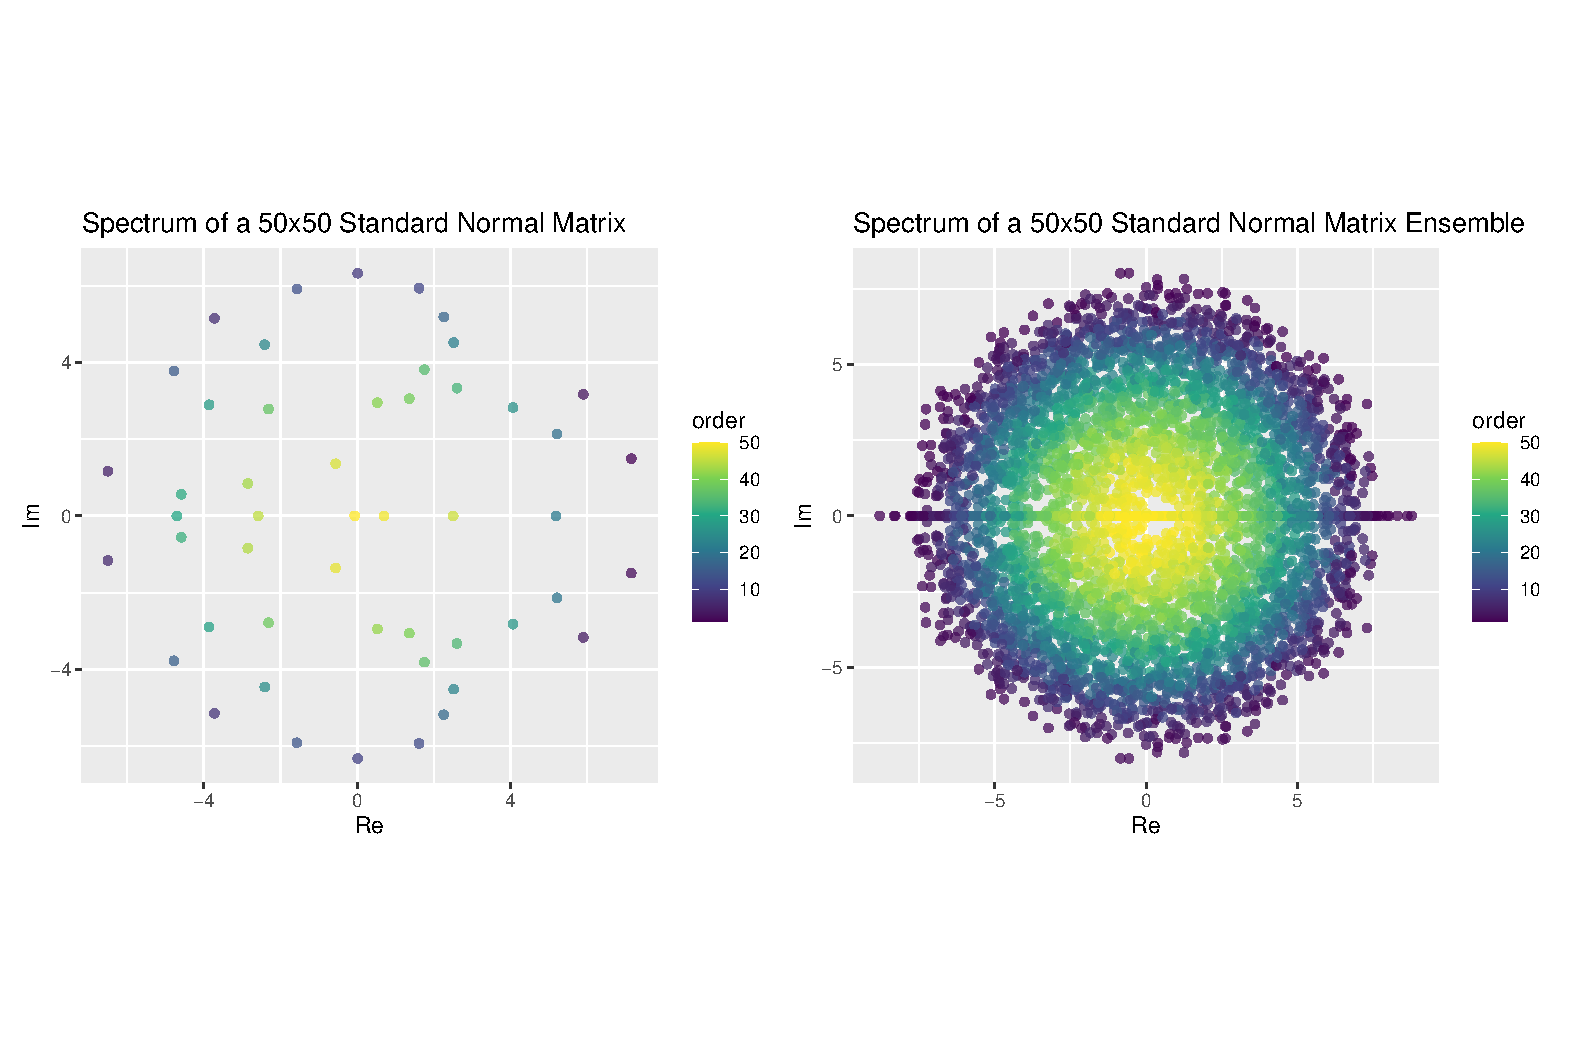
\includegraphics[scale = #2]{../graphics/chap2/2-1-2_comparison}
    \caption{Spectrum of a Matrix versus an Ensemble}
   \end{center}
   \label{ensemble_comparison_plot}
  \end{figure}
}

%%%%%%%%%%%%%%%%%%%%%%%%%%%%%%%%%%%%%%%%%%%%%%%%%%%%%%%%%%%%%%%%%%%%%%%%%%%%%%%%%%%%%%%%%%
%                                 Section 2
%%%%%%%%%%%%%%%%%%%%%%%%%%%%%%%%%%%%%%%%%%%%%%%%%%%%%%%%%%%%%%%%%%%%%%%%%%%%%%%%%%%%%%%%%%

\newcommand{\FIGUREorderscheme}[2]{
  \begin{figure}[#1]
   \begin{center}
    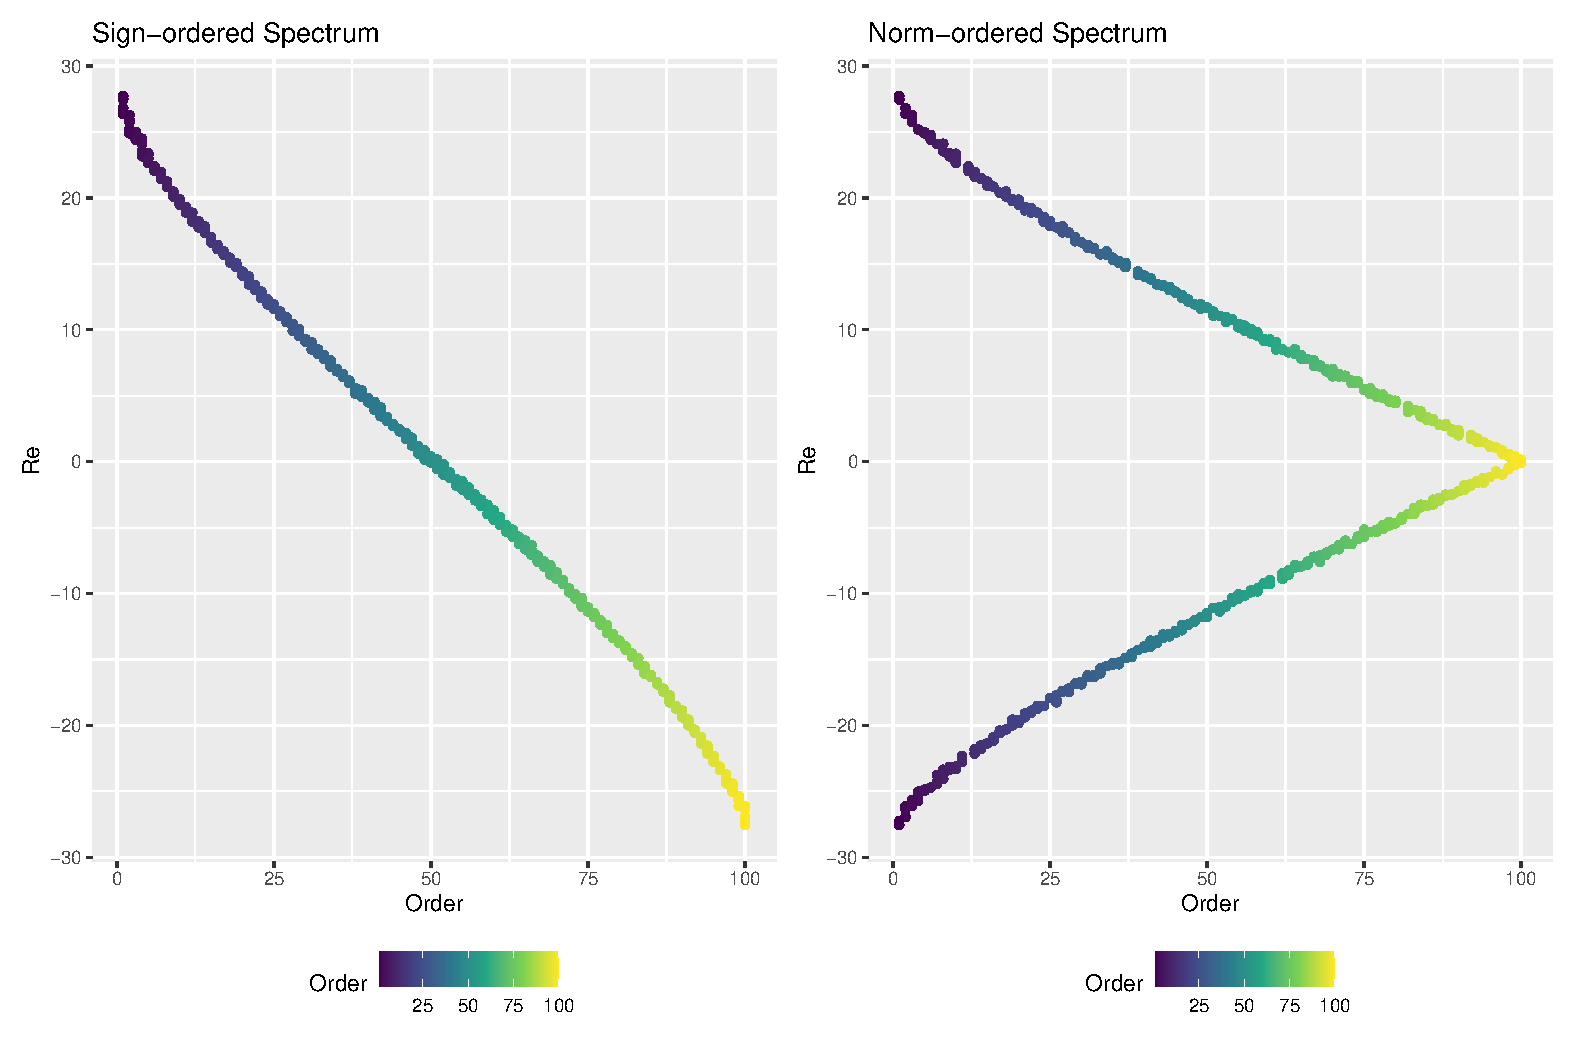
\includegraphics[scale = #2]{../graphics/chap2/2-2-1_orderscheme}
    \caption{Spectrum displaying two different ordering scheme}
   \end{center}
   \label{orderscheme_plot}
  \end{figure}
}

%%%%%%%%%%%%%%%%%%%%%%%%%%%%%%%%%%%%%%%%%%%%%%%%%%%%%%%%%%%%%%%%%%%%%%%%%%%%%%%%%%%%%%%%%%
%                                 Section 3
%%%%%%%%%%%%%%%%%%%%%%%%%%%%%%%%%%%%%%%%%%%%%%%%%%%%%%%%%%%%%%%%%%%%%%%%%%%%%%%%%%%%%%%%%%

\newcommand{\FIGUREsymmetricspectrum}[2]{
  \begin{figure}[#1]
   \begin{center}
    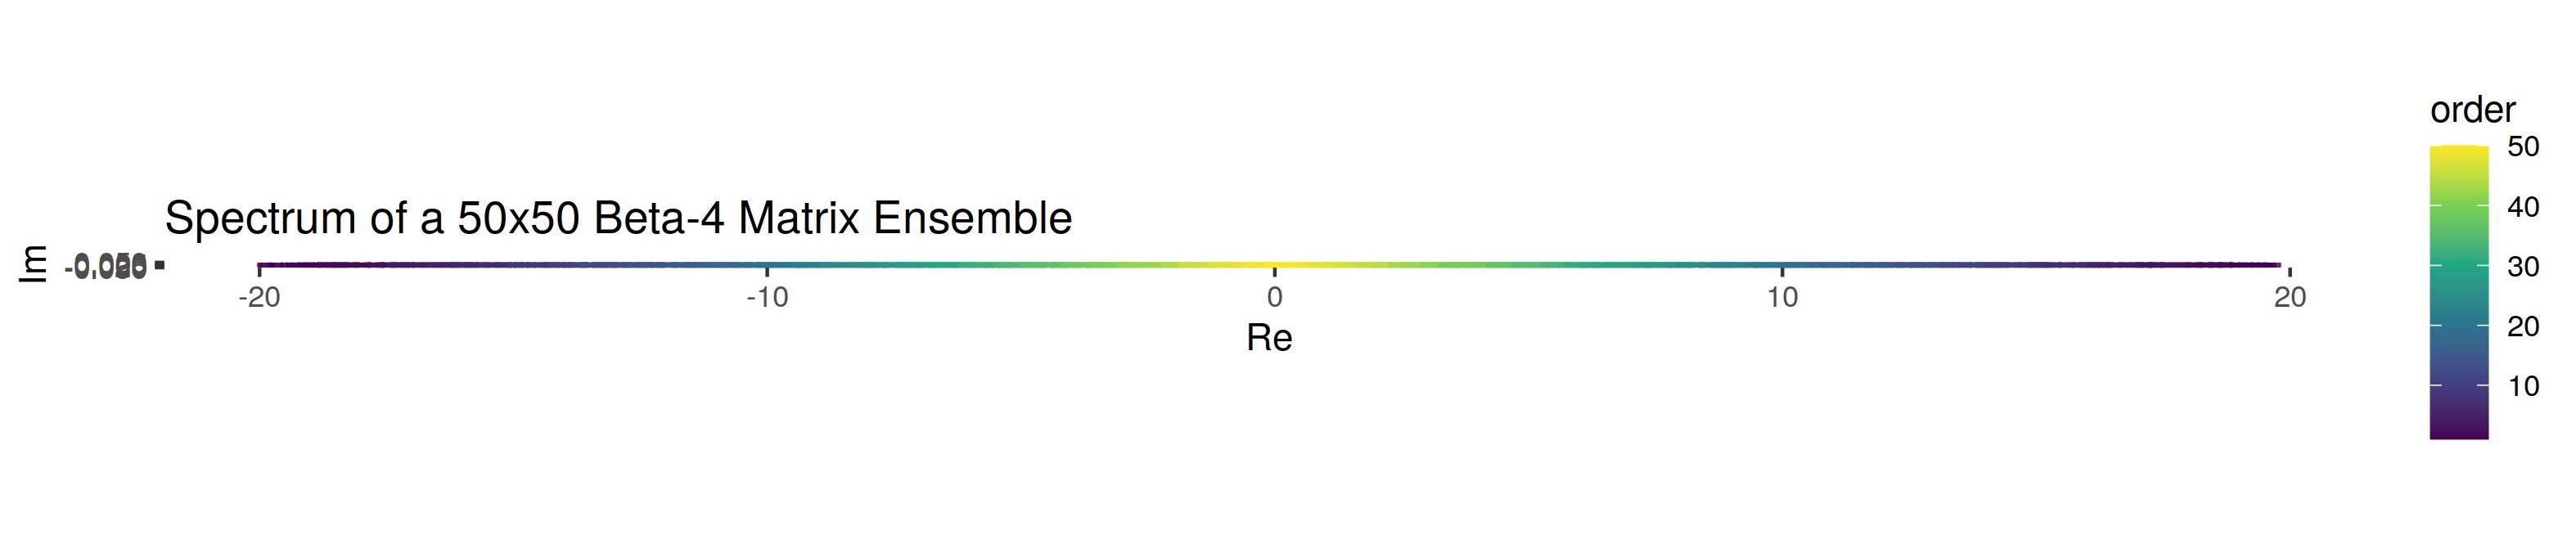
\includegraphics[scale = #2]{../graphics/chap2/2-3-1_symmetric_spectrum}
    \caption{Eigenvalues of a Symmetric Matrix are Real}
   \end{center}
   \label{symmetric_spectrum_plot}
  \end{figure}
}

\newcommand{\FIGUREsemicircle}[2]{
  \begin{figure}[#1]
   \begin{center}
    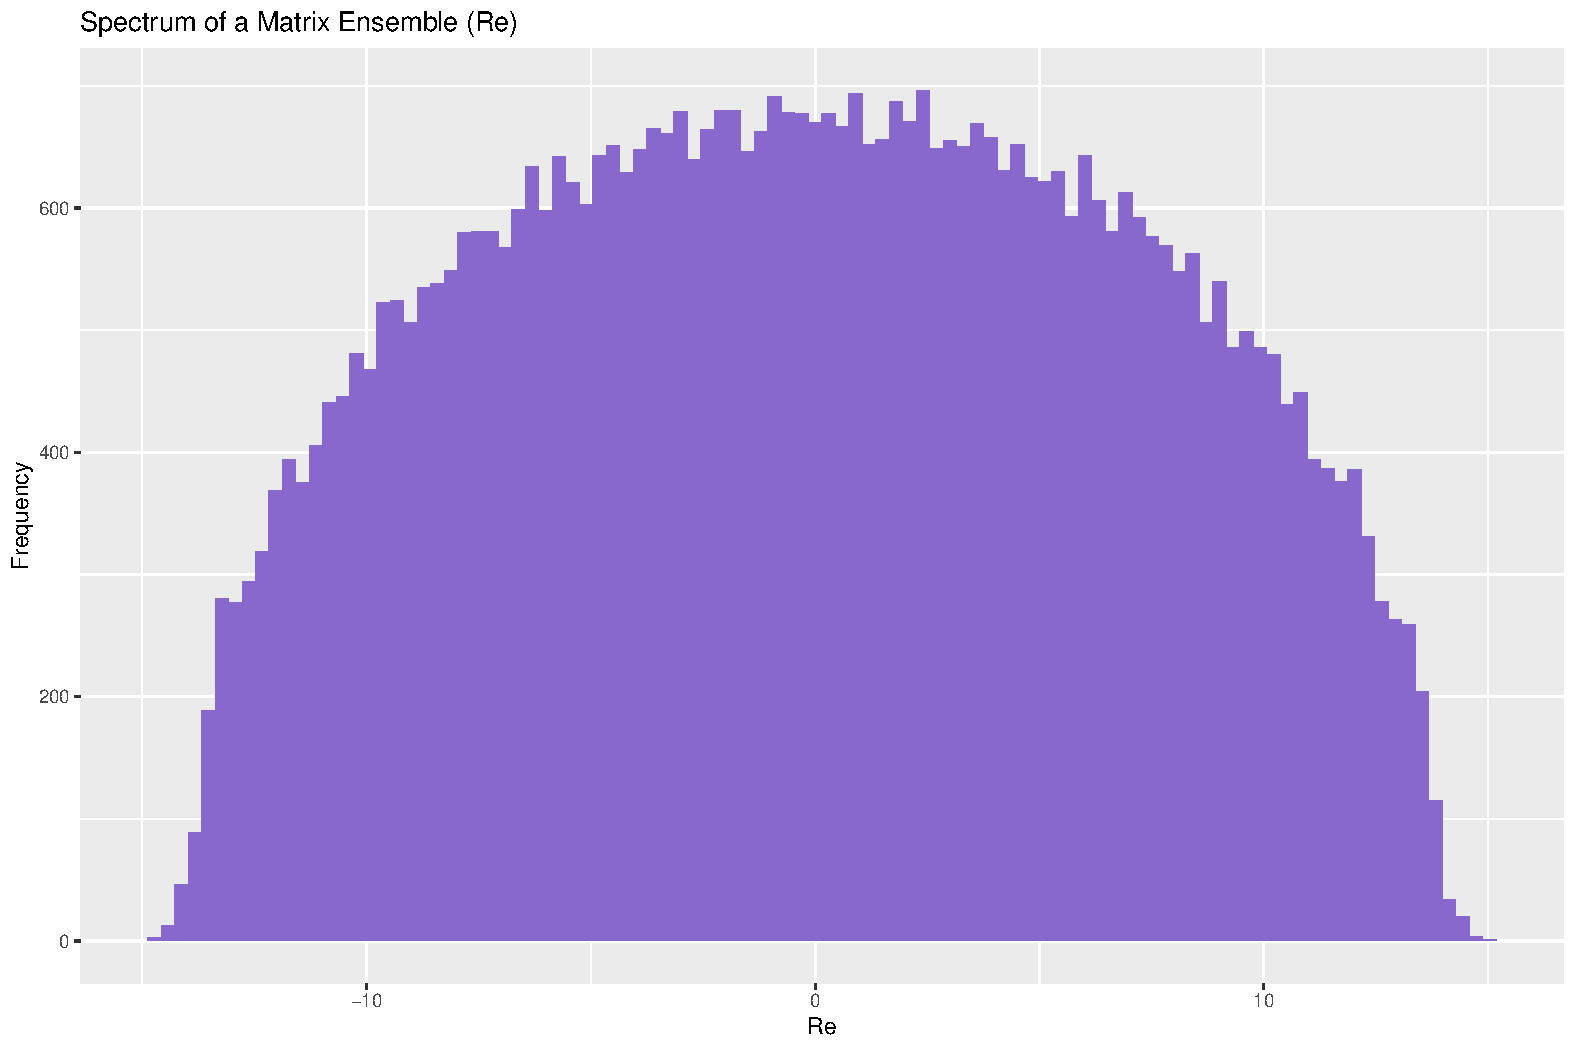
\includegraphics[scale = #2]{../graphics/chap2/2-3-2_semicircle}
    \caption{Eigenvalues of a Symmetric Matrix displaying the Semicircle Distribution}
   \end{center}
   \label{semicircle_plot}
  \end{figure}
}

%%%%%%%%%%%%%%%%%%%%%%%%%%%%%%%%%%%%%%%%%%%%%%%%%%%%%%%%%%%%%%%%%%%%%%%%%%%%%%%%%%%%%%%%%%
%                                 Section 4
%%%%%%%%%%%%%%%%%%%%%%%%%%%%%%%%%%%%%%%%%%%%%%%%%%%%%%%%%%%%%%%%%%%%%%%%%%%%%%%%%%%%%%%%%%

\newcommand{\FIGUREunifspectrum}[2]{
  \begin{figure}[#1]
   \begin{center}
    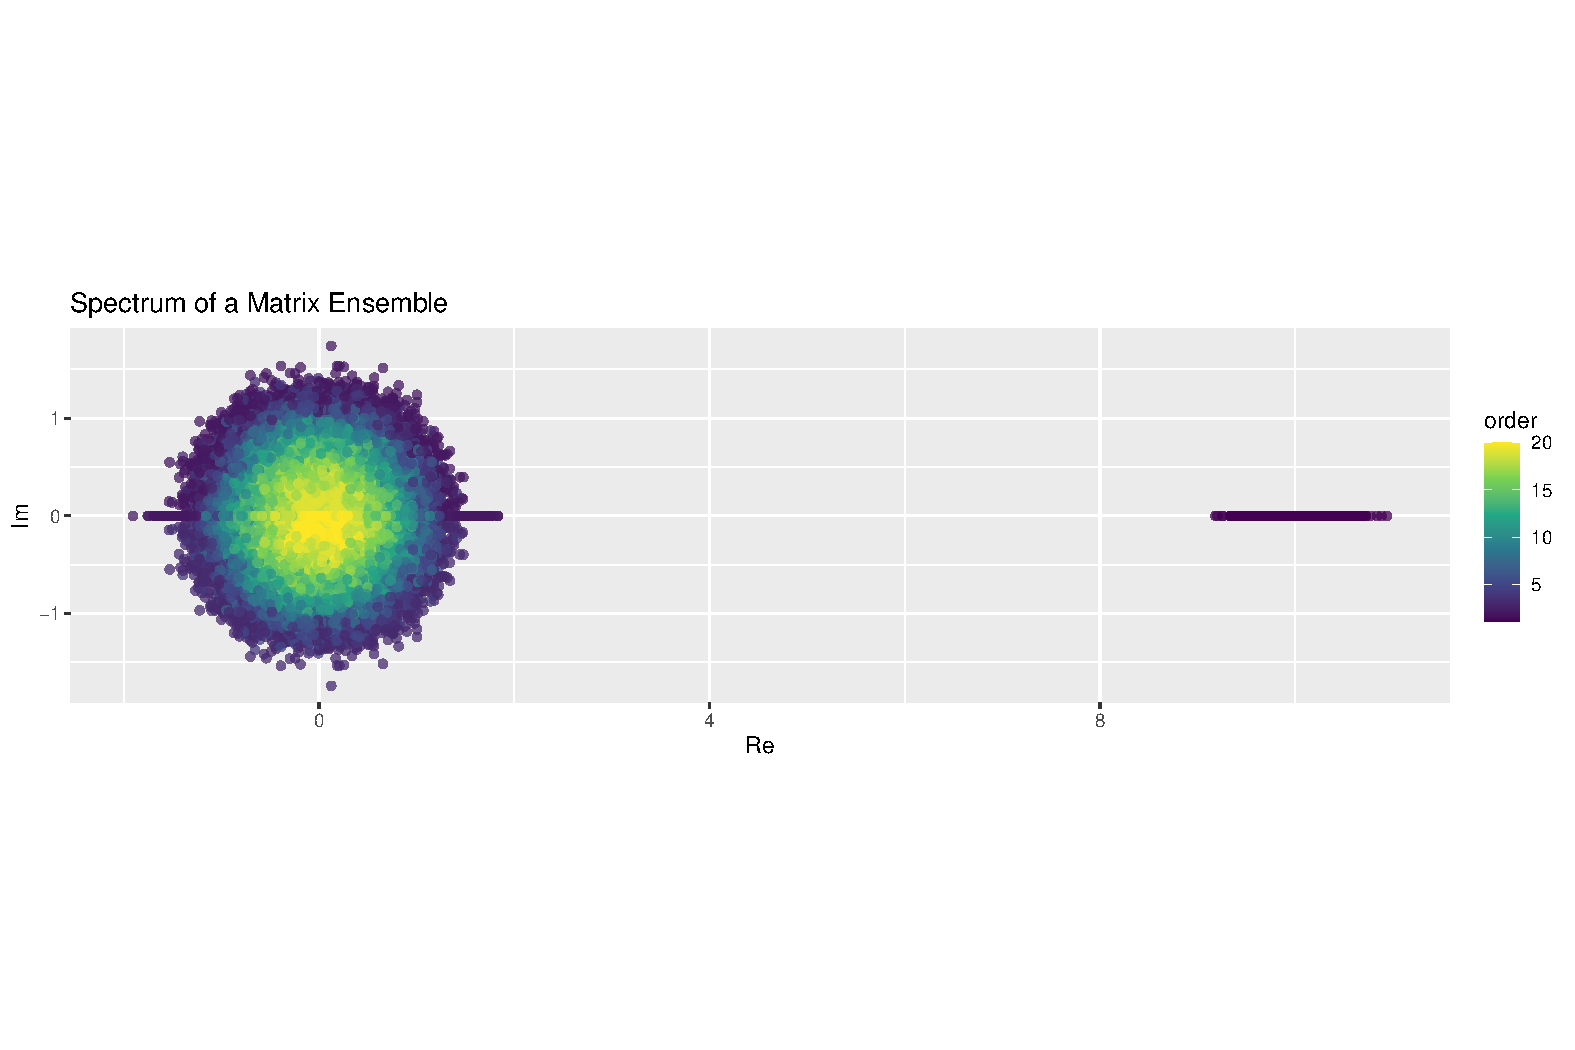
\includegraphics[scale = #2]{../graphics/chap2/2-4_unif01_spec}
    \caption{Spectrum of a Unif(0,1) ensemble}
   \end{center}
   \label{spectrum_unif_ensemble_plot}
  \end{figure}
}

\newcommand{\FIGUREnormalspectrum}[2]{
  \begin{figure}[#1]
   \begin{center}
    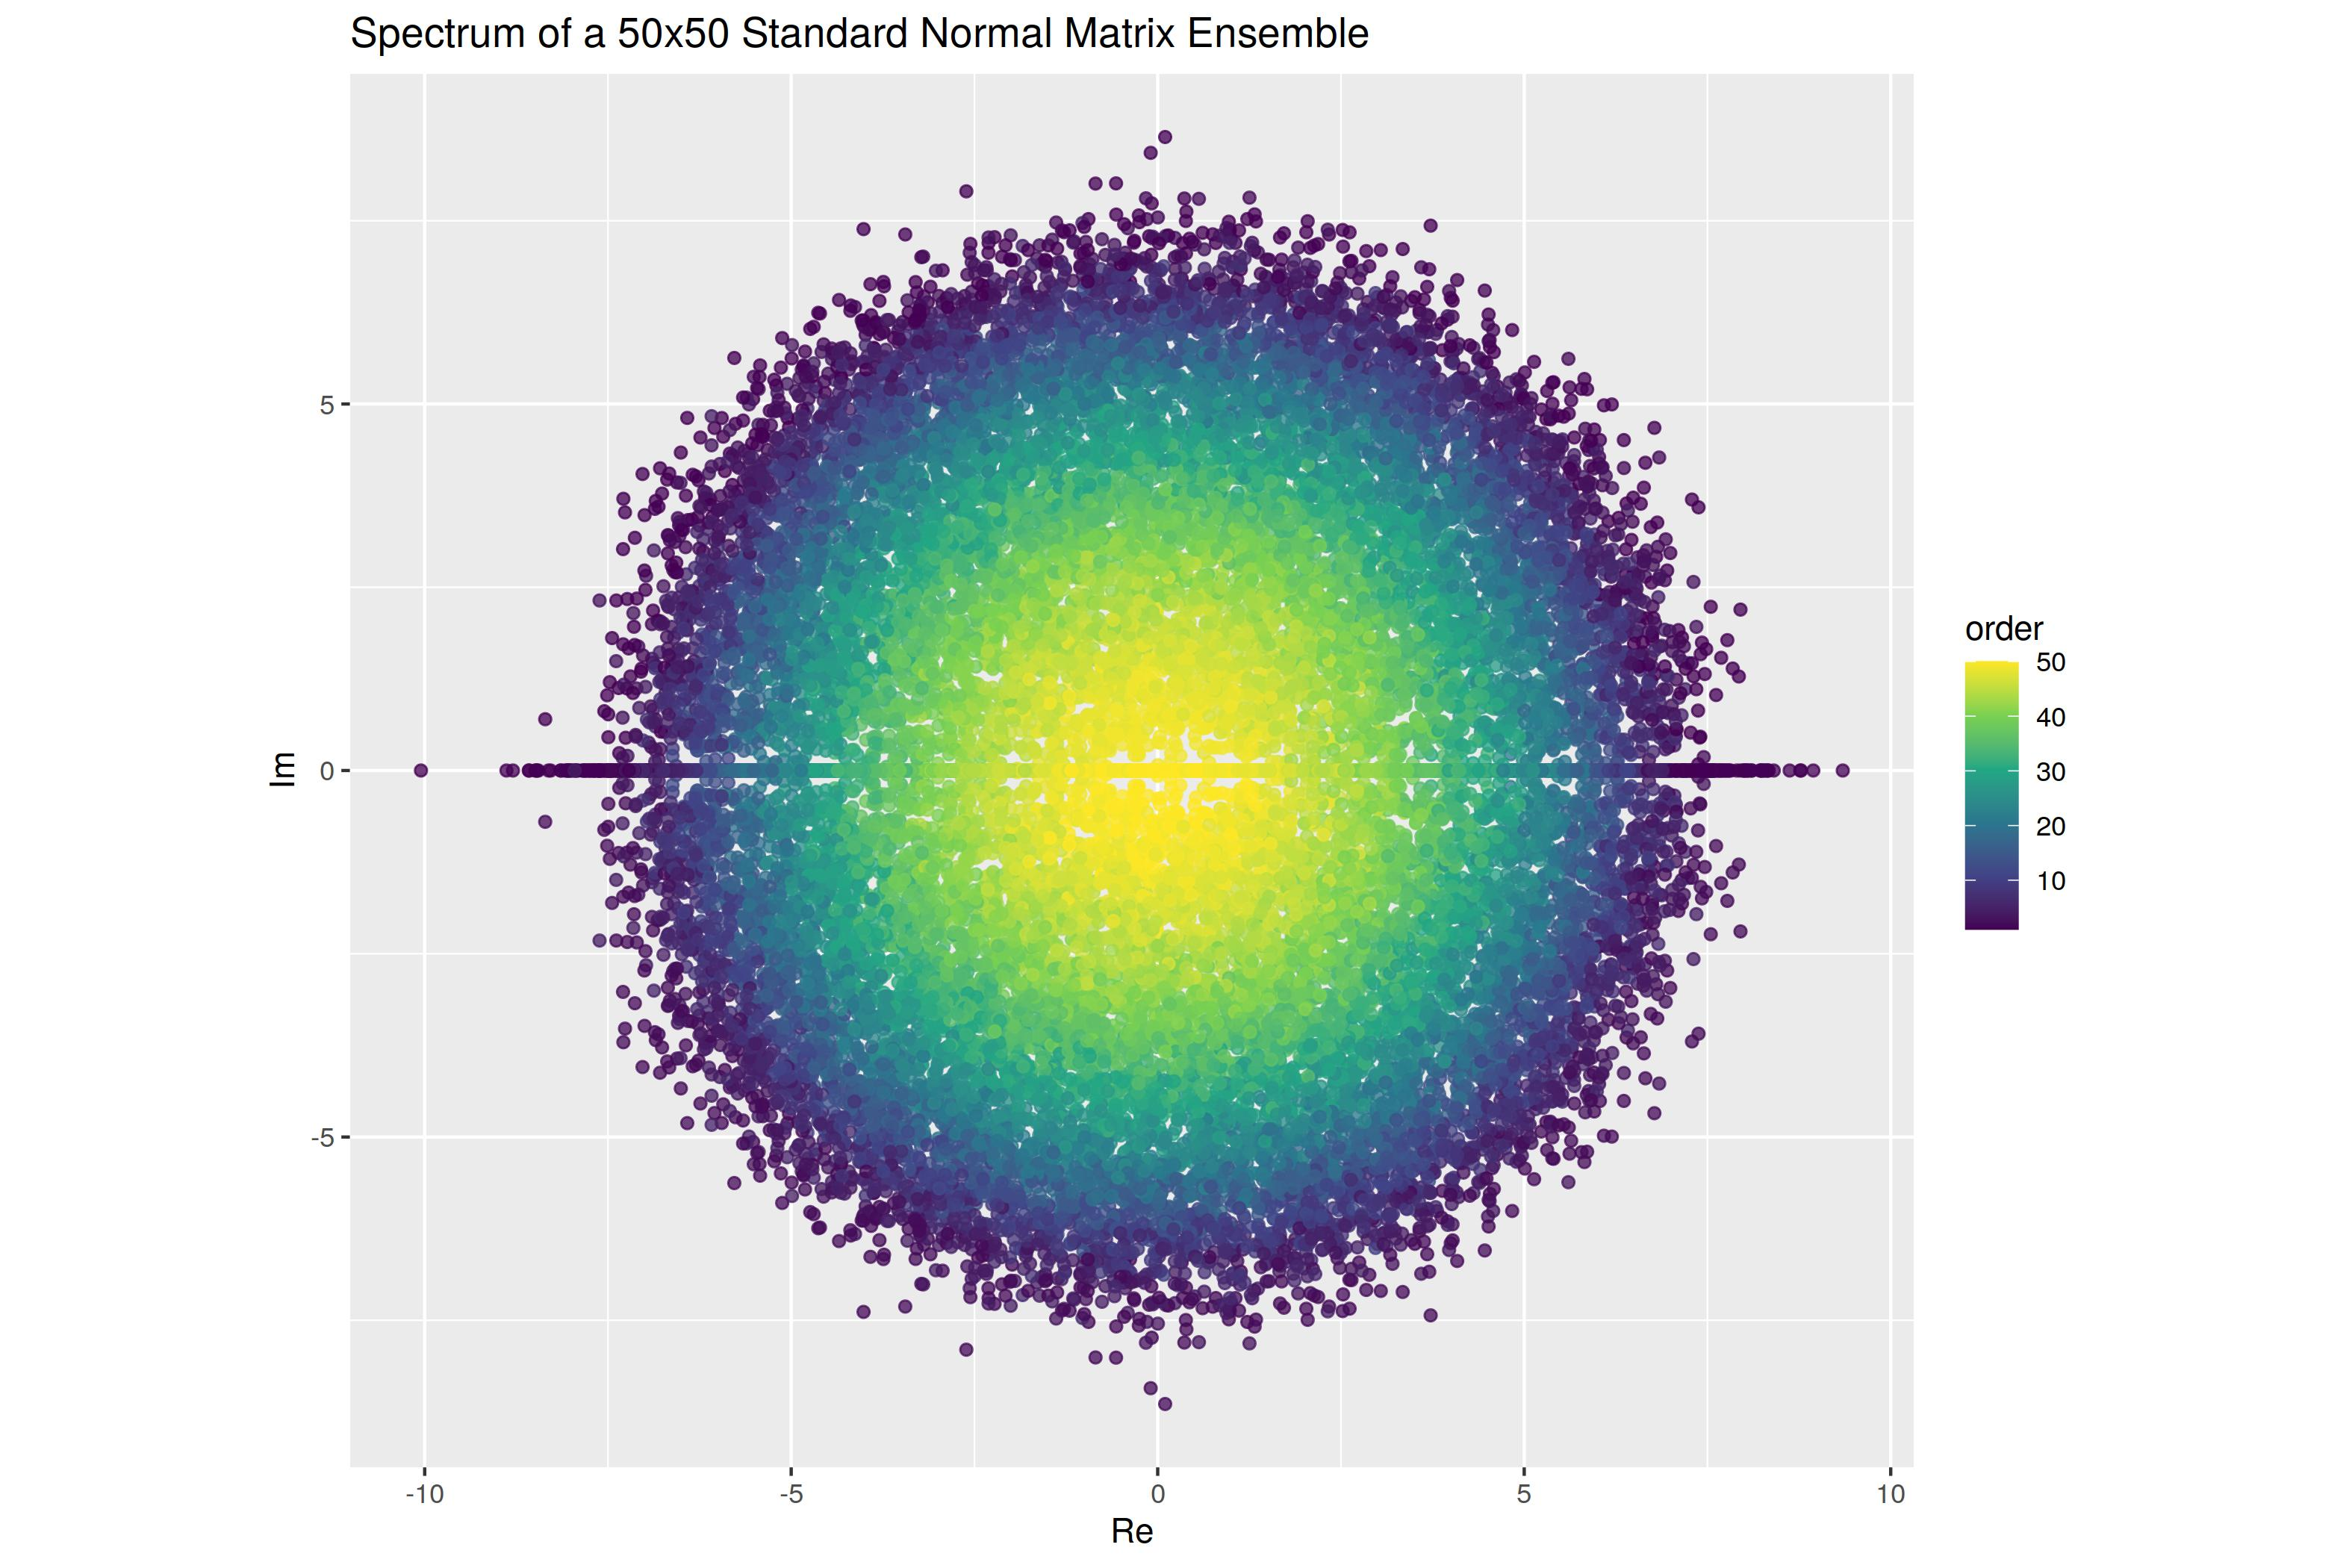
\includegraphics[scale = #2]{../graphics/chap2/2-4_normal_spec}
    \caption{Spectrum of a Standard Normal Matrix ensemble}
   \end{center}
   \label{spectrum_normal_ensemble_plot}
  \end{figure}
}

\newcommand{\FIGUREnormalCPLXHERMspectrum}[2]{
  \begin{figure}[#1]
   \begin{center}
    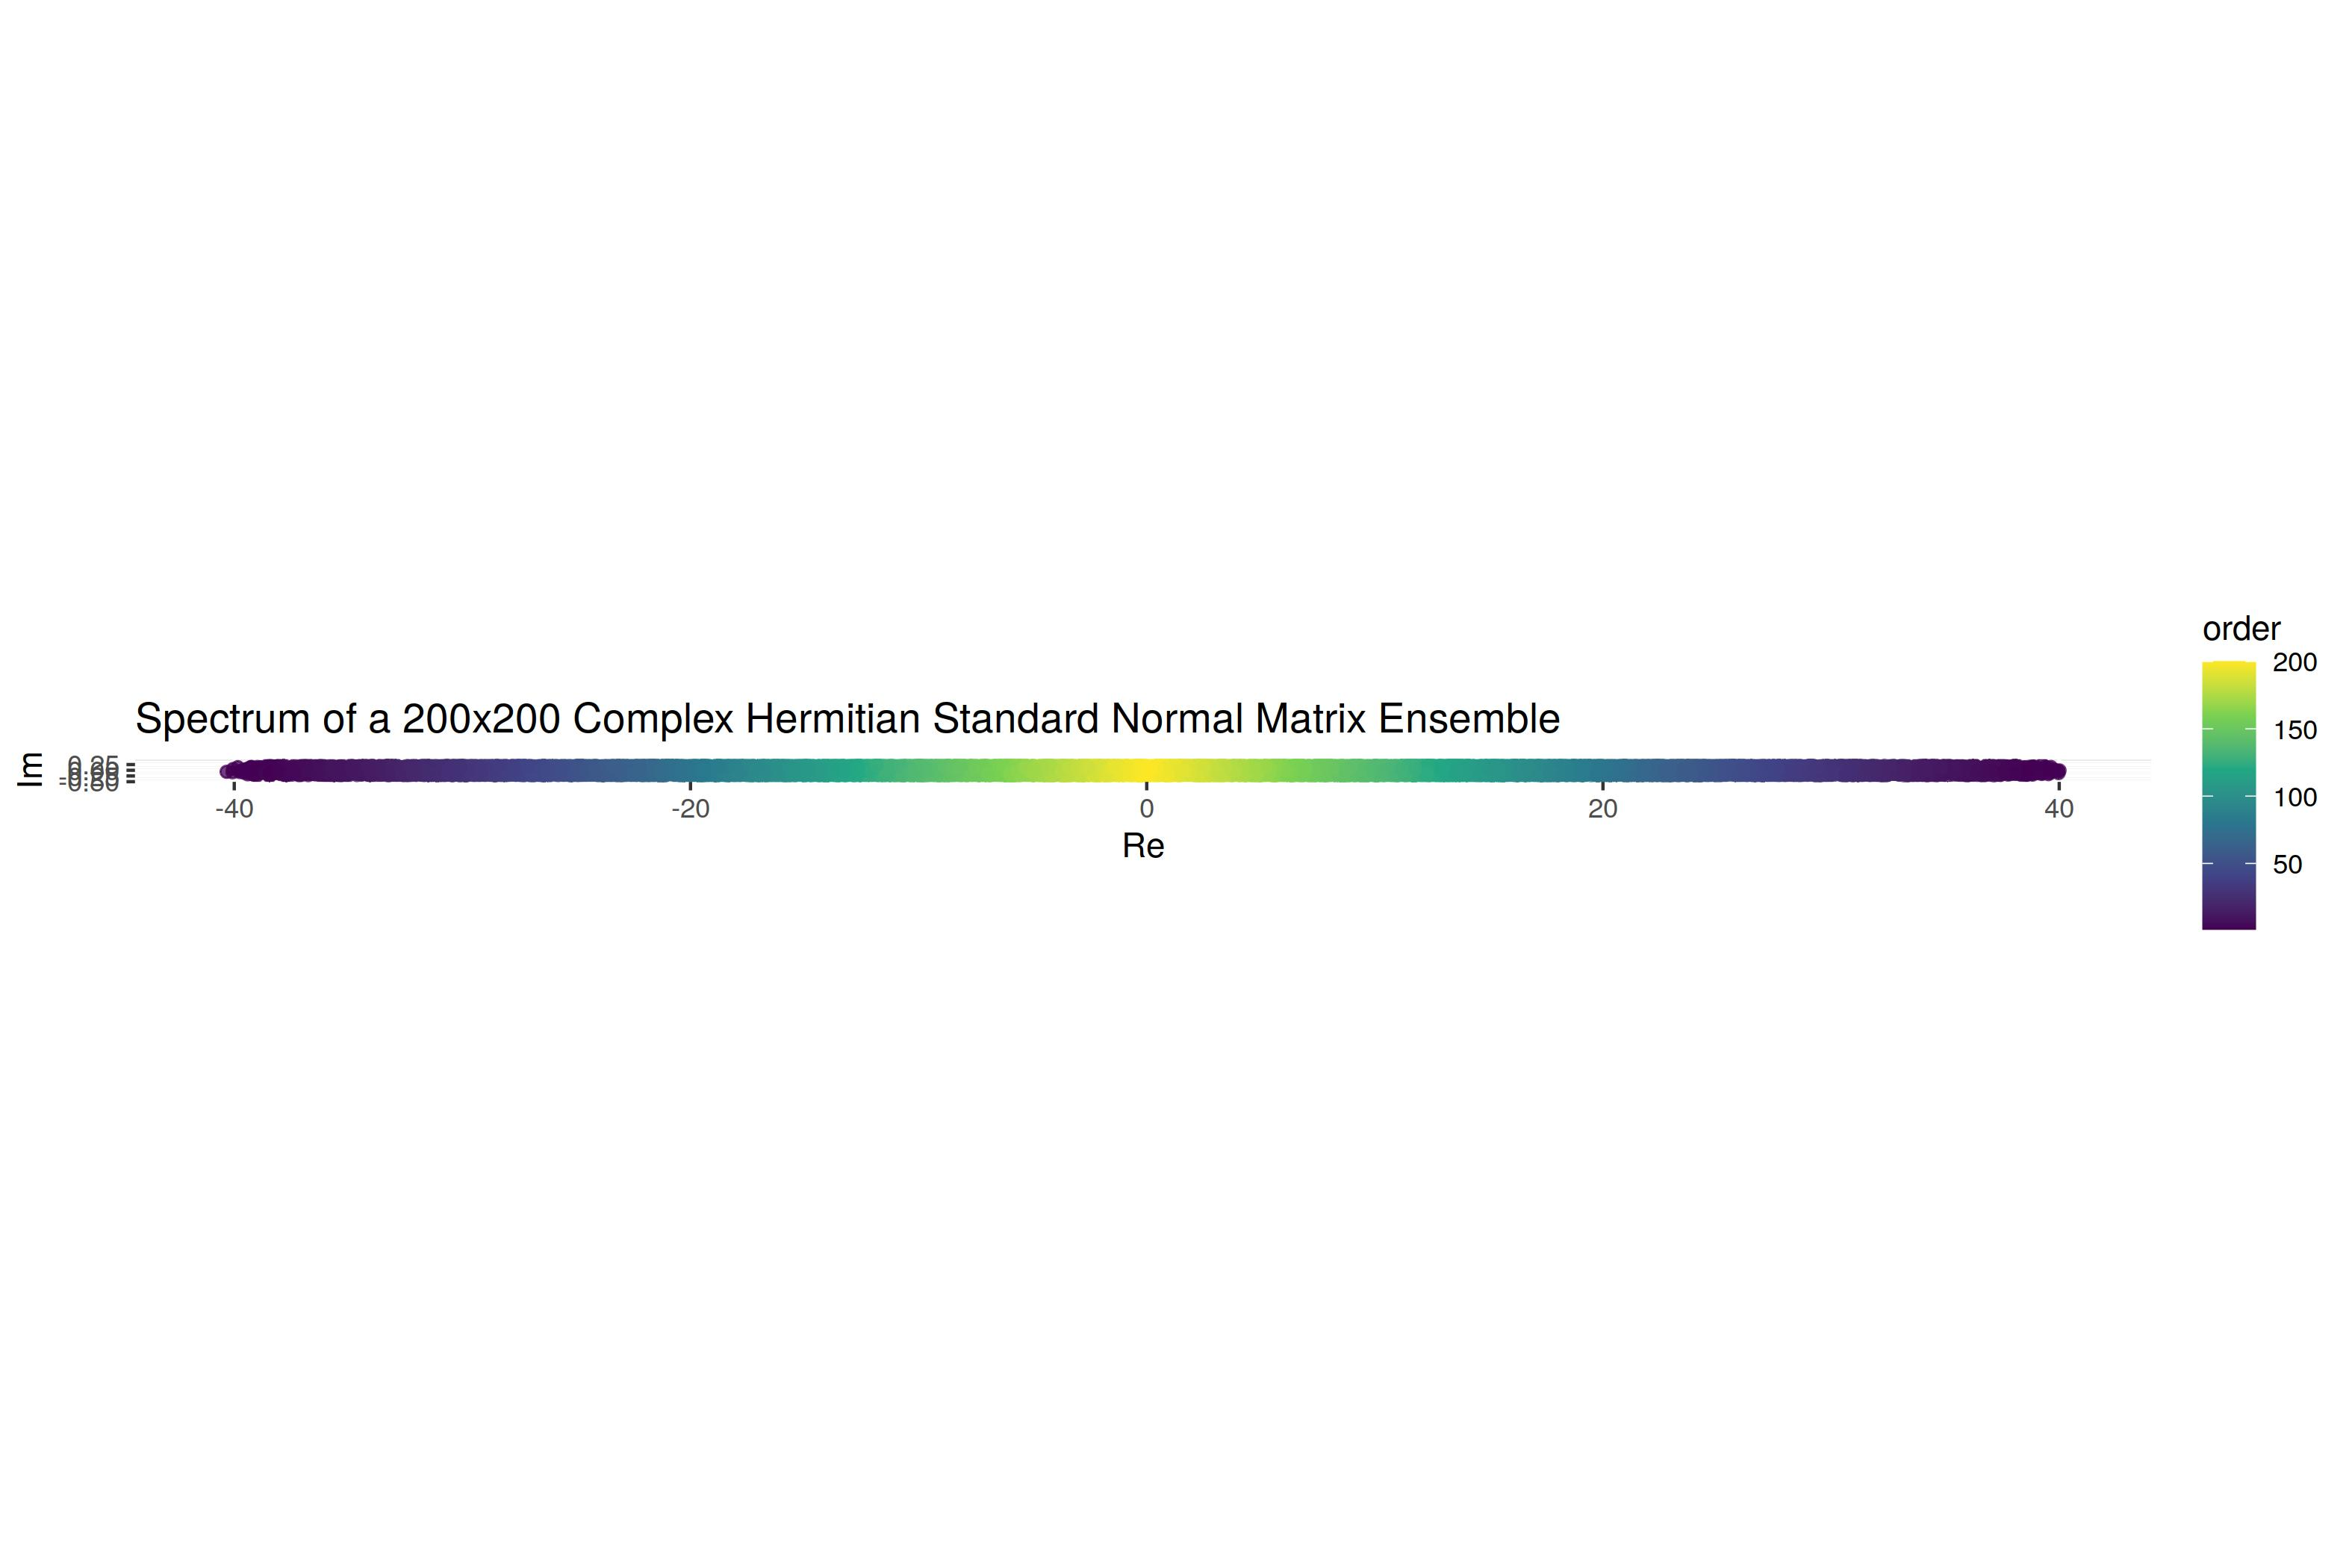
\includegraphics[scale = #2]{../graphics/chap2/2-4_cplxherm_normal_spec}
    \caption{Spectrum of a Complex Hermitian Standard Normal Matrix ensemble}
   \end{center}
   \label{spectrum_cplxherm_normal_ensemble_plot}
  \end{figure}
}

\newcommand{\FIGUREstochspectrum}[2]{
  \begin{figure}[#1]
   \begin{center}
    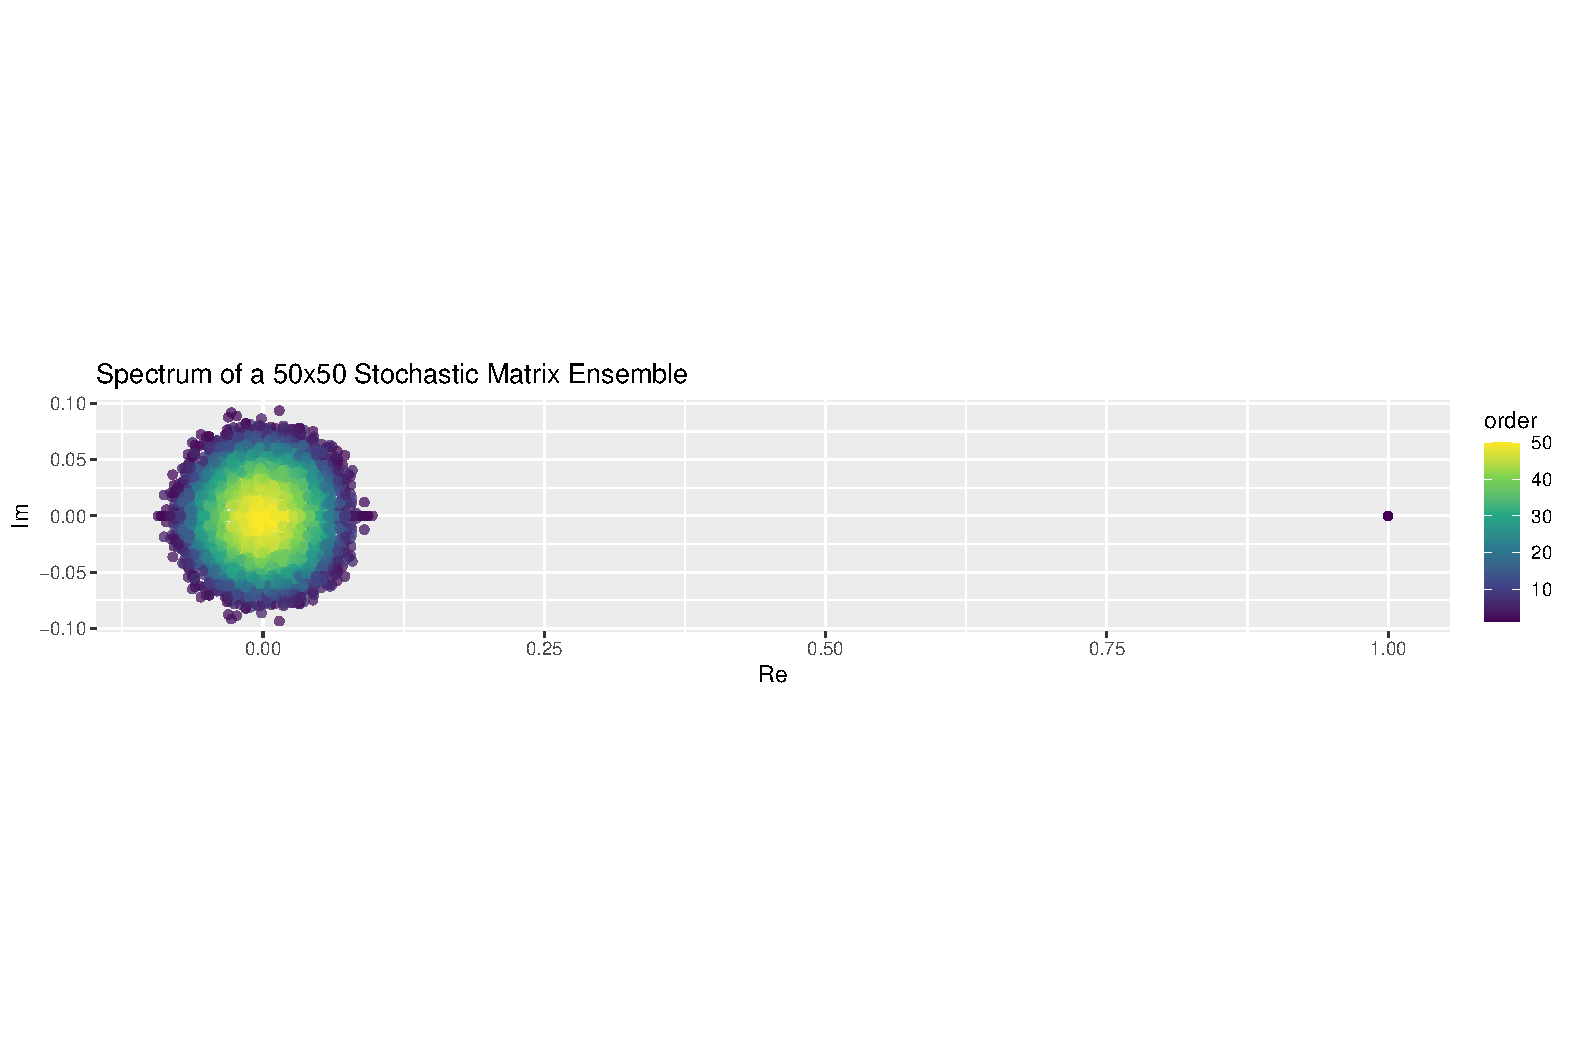
\includegraphics[scale = #2]{../graphics/chap2/2-4_stoch_spec}
    \caption{Spectrum of a Stochastic Matrix ensemble}
   \end{center}
   \label{spectrum_stoch_ensemble_plot}
  \end{figure}
}

\newcommand{\FIGUREsymmstochspectrum}[2]{
  \begin{figure}[#1]
   \begin{center}
    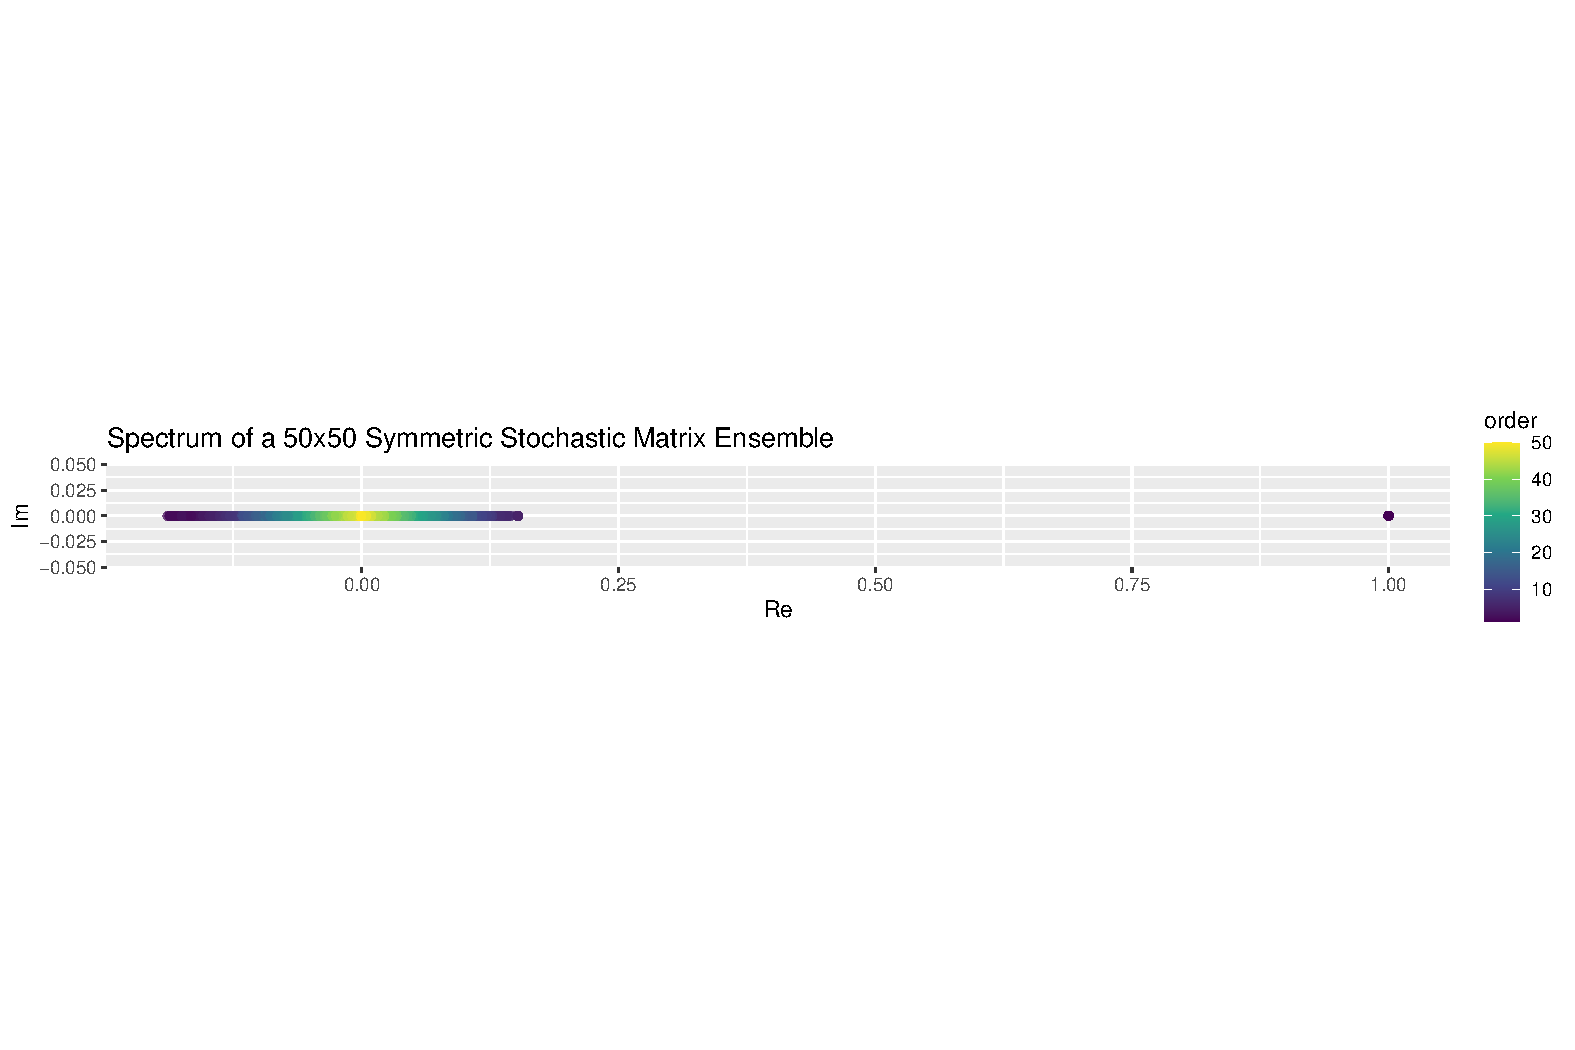
\includegraphics[scale = #2]{../graphics/chap2/2-4_symmstoch_spec}
    \caption{Spectrum of a Symmetric Stochastic Matrix ensemble}
   \end{center}
   \label{spectrum_stoch_ensemble_plot}
  \end{figure}
}

\newcommand{\FIGUREerdosLAMTWO}[2]{
  \begin{figure}[#1]
   \begin{center}
    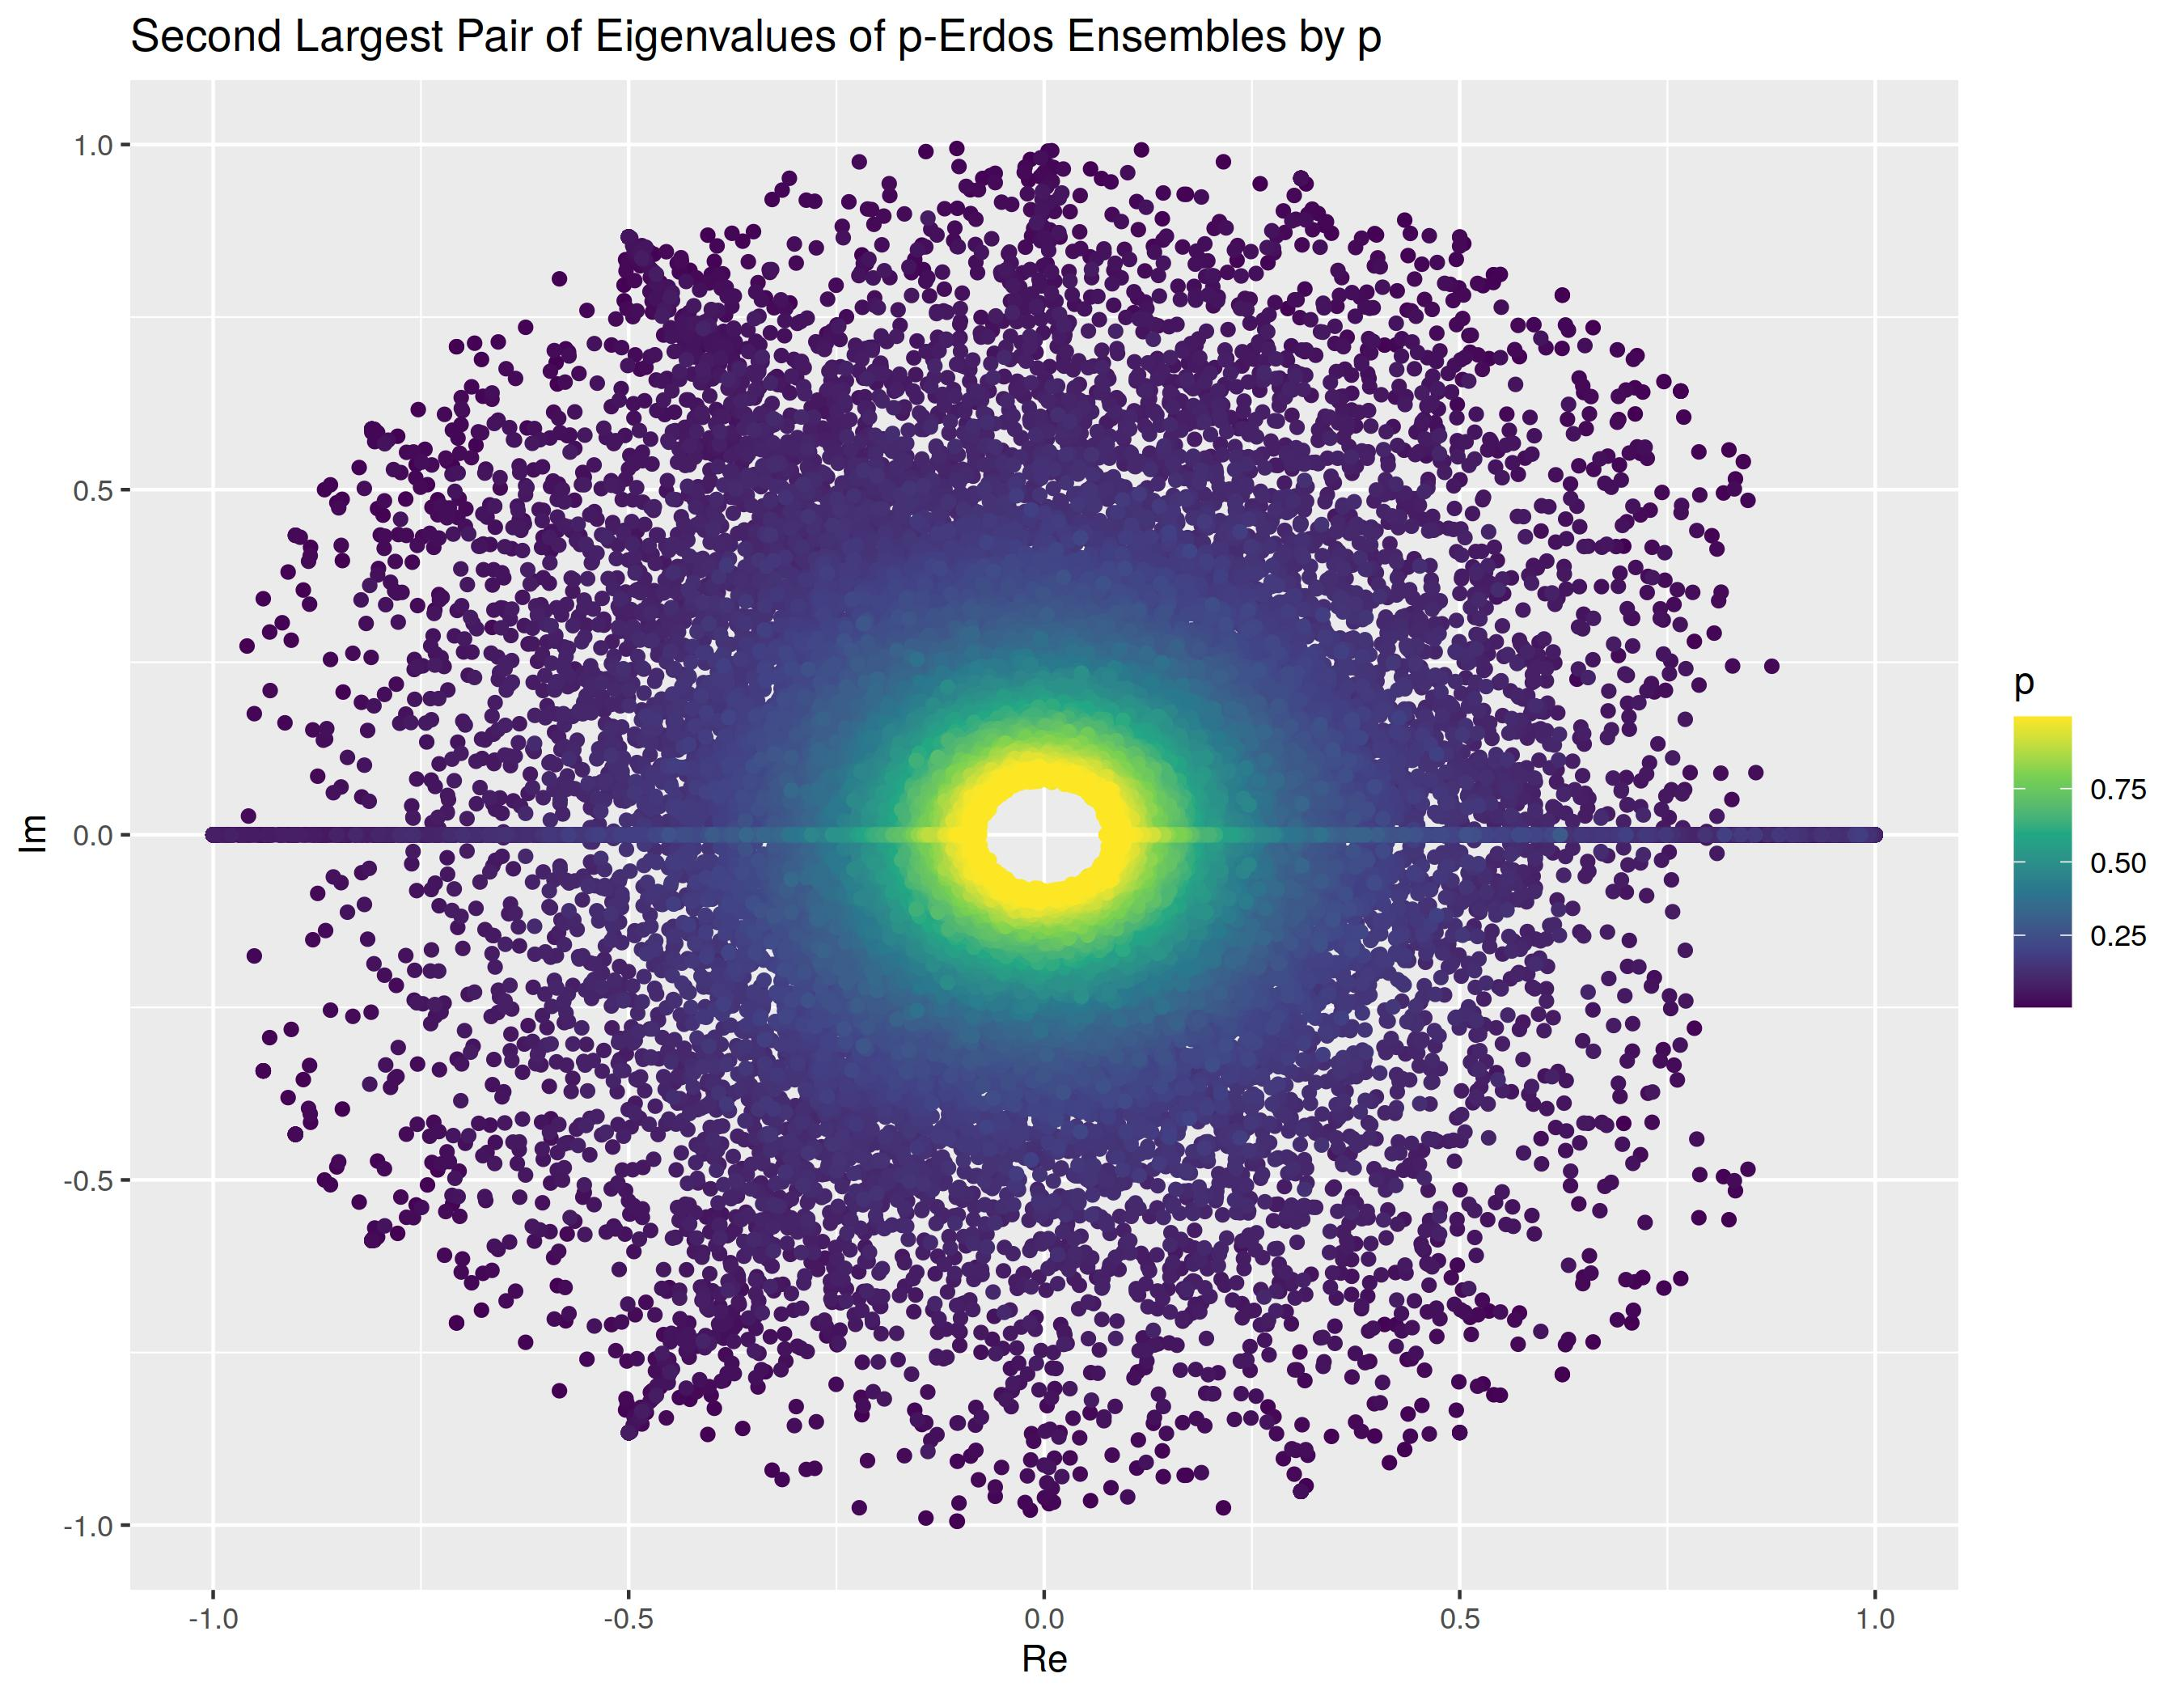
\includegraphics[scale = #2]{../graphics/chap2/2-4_erdos_lam2}
    \caption{2nd Largest Eigenvalue of an Erdos-p ensemble}
   \end{center}
   \label{spectrum_erdoslam2_plot}
  \end{figure}
}

%%%%%%%%%%%%%%%%%%%%%%%%%%%%%%%%%%%%%%%%%%%%%%%%%%%%%%%%%%%%%%%%%%%%%%%%%%%%%%%%%%%%%%%%%%
%                                  CHAPTER 3
%%%%%%%%%%%%%%%%%%%%%%%%%%%%%%%%%%%%%%%%%%%%%%%%%%%%%%%%%%%%%%%%%%%%%%%%%%%%%%%%%%%%%%%%%%

%%%%%%%%%%%%%%%%%%%%%%%%%%%%%%%%%%%%%%%%%%%%%%%%%%%%%%%%%%%%%%%%%%%%%%%%%%%%%%%%%%%%%%%%%%
%                                 Section 3
%%%%%%%%%%%%%%%%%%%%%%%%%%%%%%%%%%%%%%%%%%%%%%%%%%%%%%%%%%%%%%%%%%%%%%%%%%%%%%%%%%%%%%%%%%

\newcommand{\FIGUREwignerbeta}[2]{
  \begin{figure}[#1]
   \begin{center}
    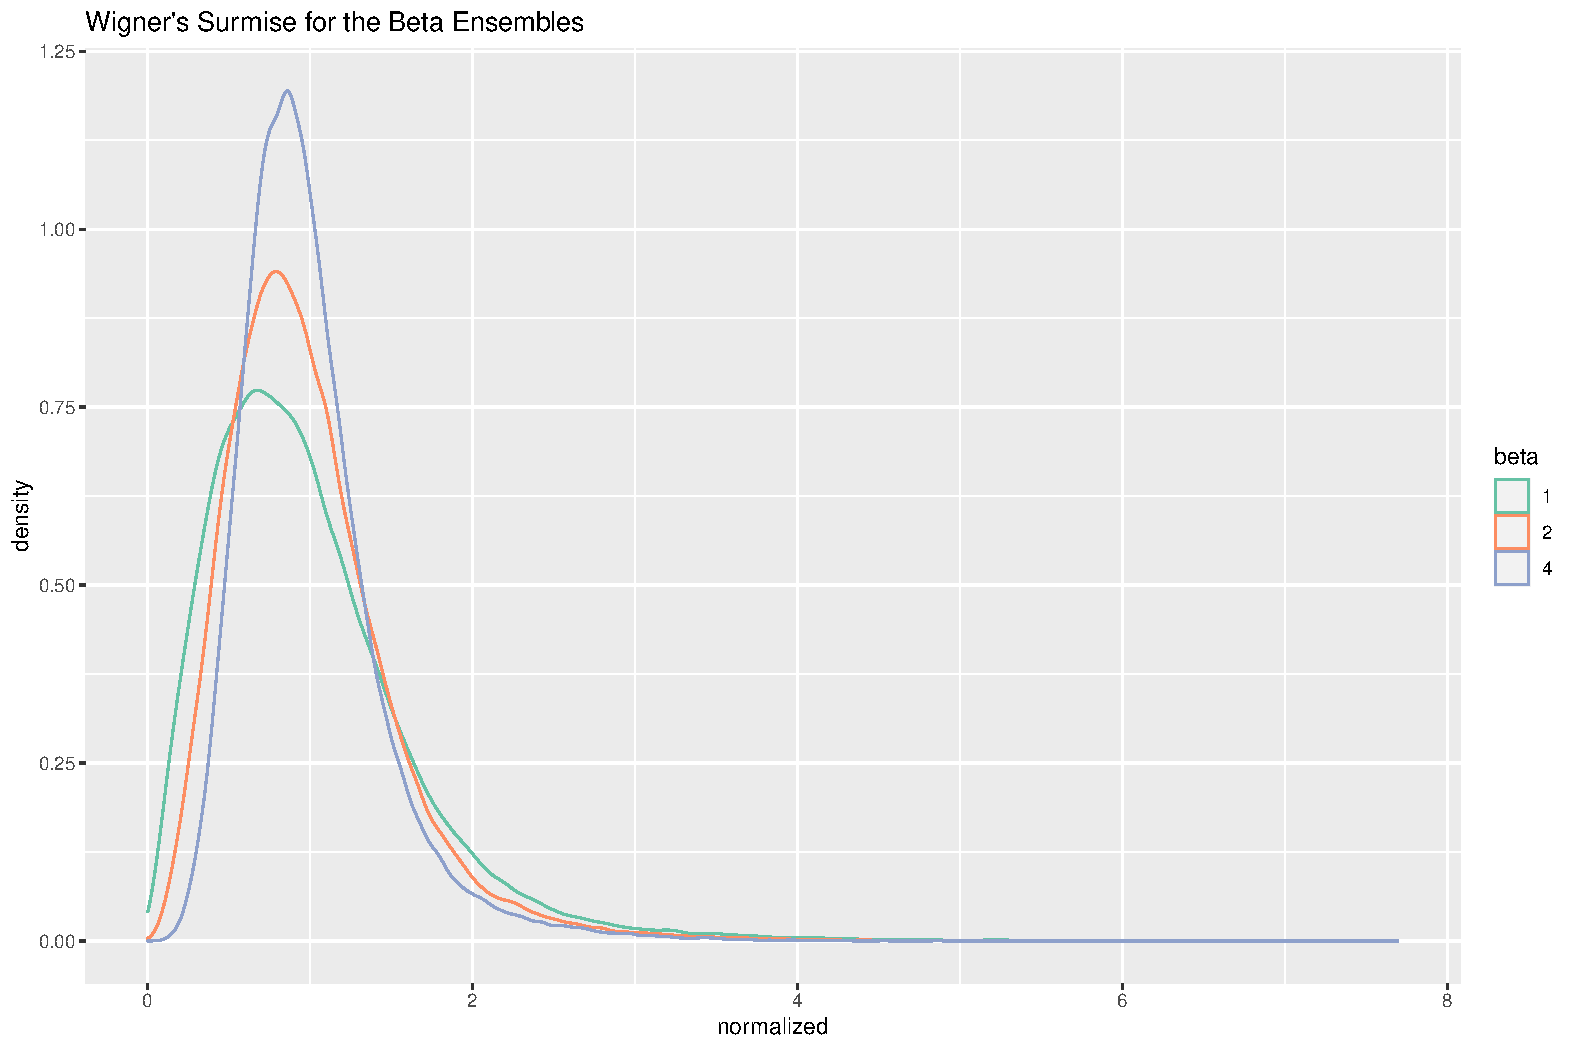
\includegraphics[scale = #2]{../graphics/chap3/3-3_wigner_beta}
    \caption{Wigner's Surmise for standard Beta Ensembles}
   \end{center}
   \label{wigner_beta}
  \end{figure}
}

\newcommand{\FIGUREwignerbetaextended}[2]{
  \begin{figure}[#1]
   \begin{center}
    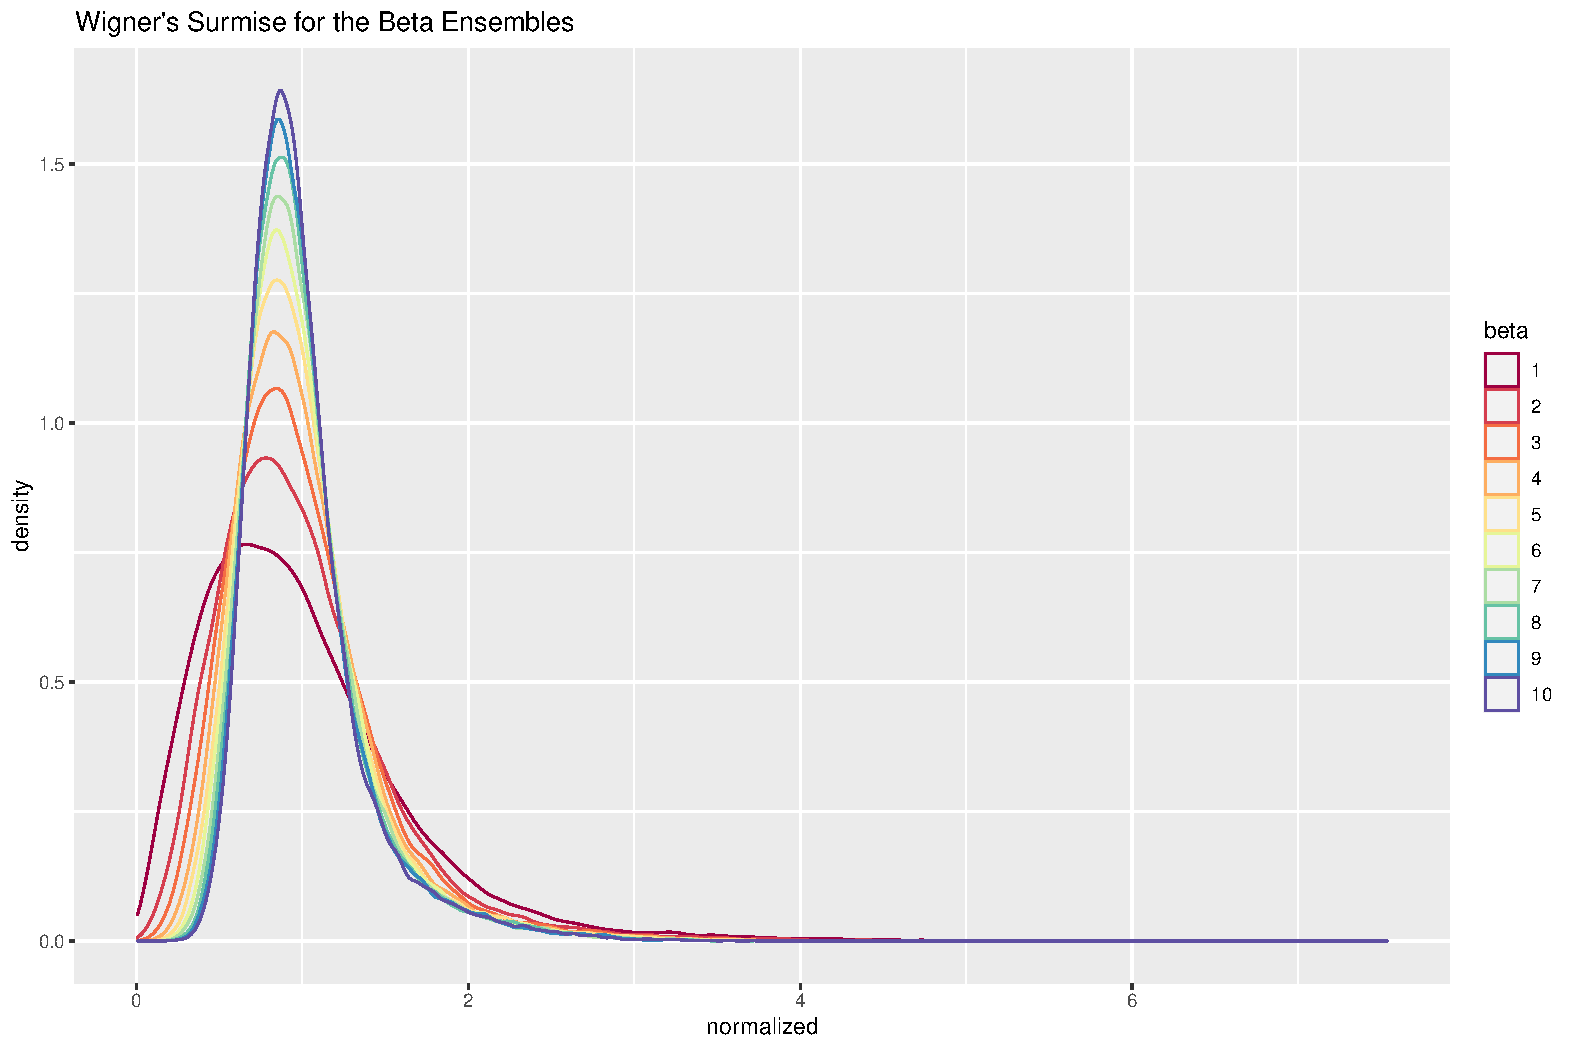
\includegraphics[scale = #2]{../graphics/chap3/3-3_wigner_beta_extended}
    \caption{Wigner's Surmise for non-standard Beta Ensembles}
   \end{center}
   \label{wigner_beta_extended}
  \end{figure}
}

%%%%%%%%%%%%%%%%%%%%%%%%%%%%%%%%%%%%%%%%%%%%%%%%%%%%%%%%%%%%%%%%%%%%%%%%%%%%%%%%%%%%%%%%%%
%                                  CHAPTER 4
%%%%%%%%%%%%%%%%%%%%%%%%%%%%%%%%%%%%%%%%%%%%%%%%%%%%%%%%%%%%%%%%%%%%%%%%%%%%%%%%%%%%%%%%%%

%%%%%%%%%%%%%%%%%%%%%%%%%%%%%%%%%%%%%%%%%%%%%%%%%%%%%%%%%%%%%%%%%%%%%%%%%%%%%%%%%%%%%%%%%%
%                                 Section 1
%%%%%%%%%%%%%%%%%%%%%%%%%%%%%%%%%%%%%%%%%%%%%%%%%%%%%%%%%%%%%%%%%%%%%%%%%%%%%%%%%%%%%%%%%%

%%%%%%%%%%%%%%%%%%%%%%%%%%%%%%%%%%%%%%%%%%%%%%%%%%%%%%%%%%%%%%%%%%%%%%%%%%%%%%%%%%%%%%%%%%
%                                 Section 2
%%%%%%%%%%%%%%%%%%%%%%%%%%%%%%%%%%%%%%%%%%%%%%%%%%%%%%%%%%%%%%%%%%%%%%%%%%%%%%%%%%%%%%%%%%

\newcommand{\FIGUREbetaREspec}[2]{
  \begin{figure}[#1]
   \begin{center}
    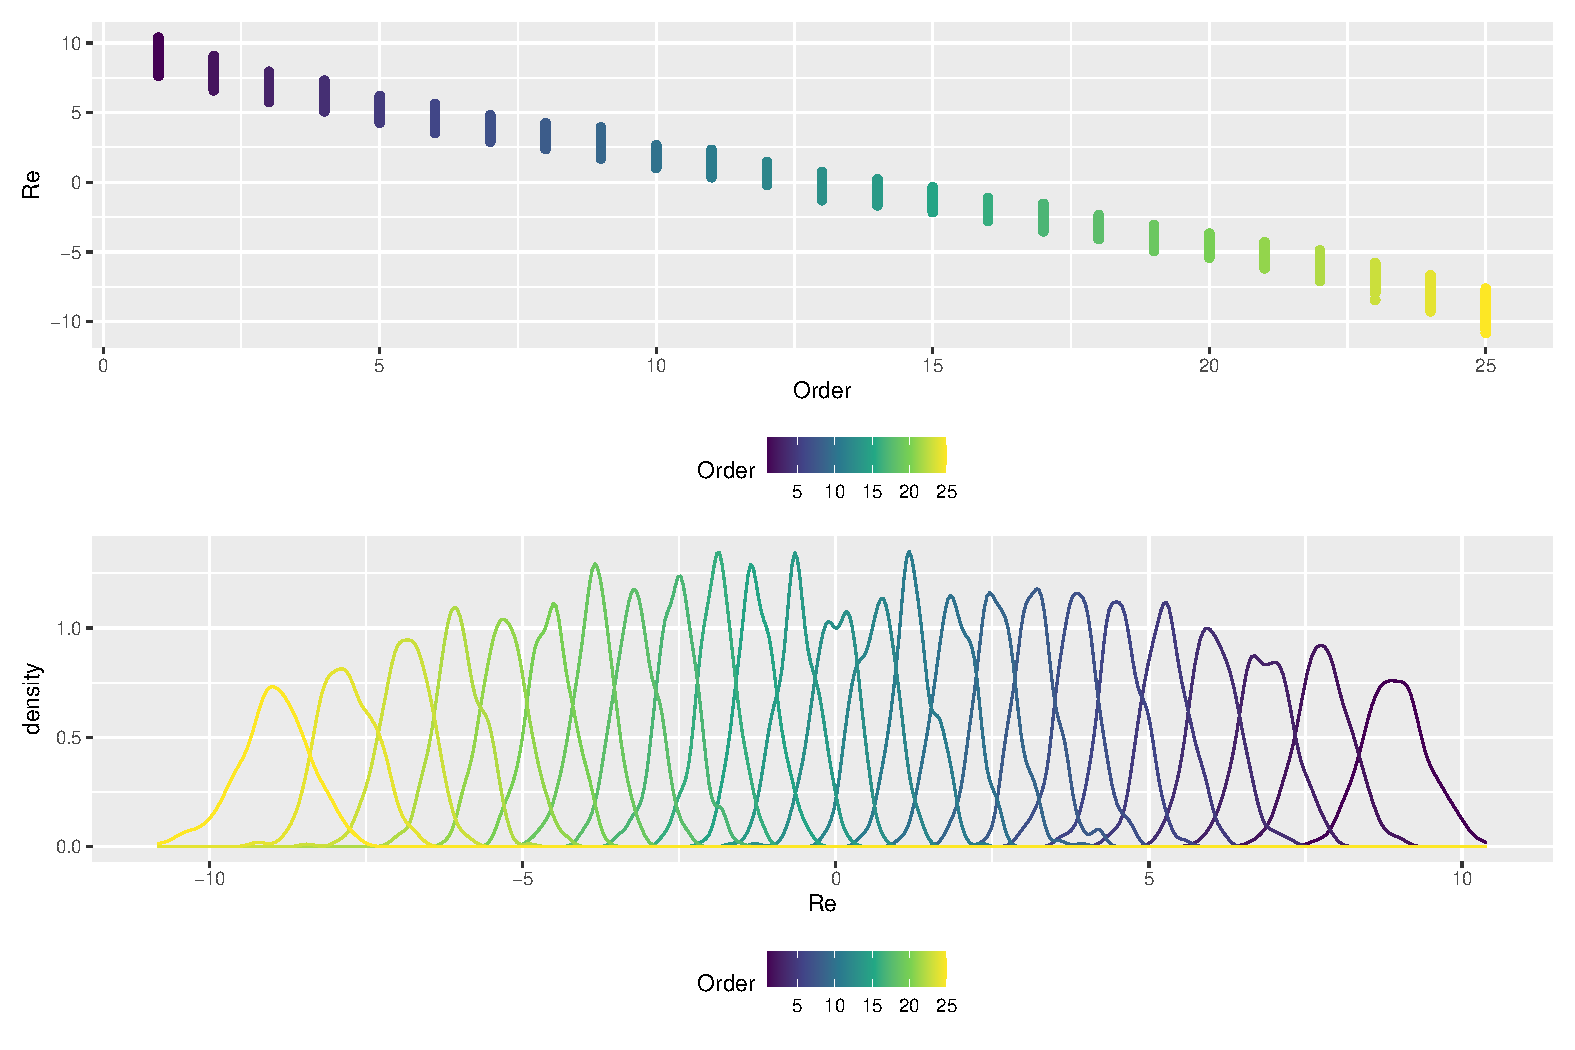
\includegraphics[scale = #2]{../graphics/chap4/4-2_Re_spec}
    \caption{Wigner's Surmise for non-standard Beta Ensembles}
   \end{center}
   \label{beta_re_spec}
  \end{figure}
}

\newcommand{\FIGUREbetaNORMspec}[2]{
  \begin{figure}[#1]
   \begin{center}
    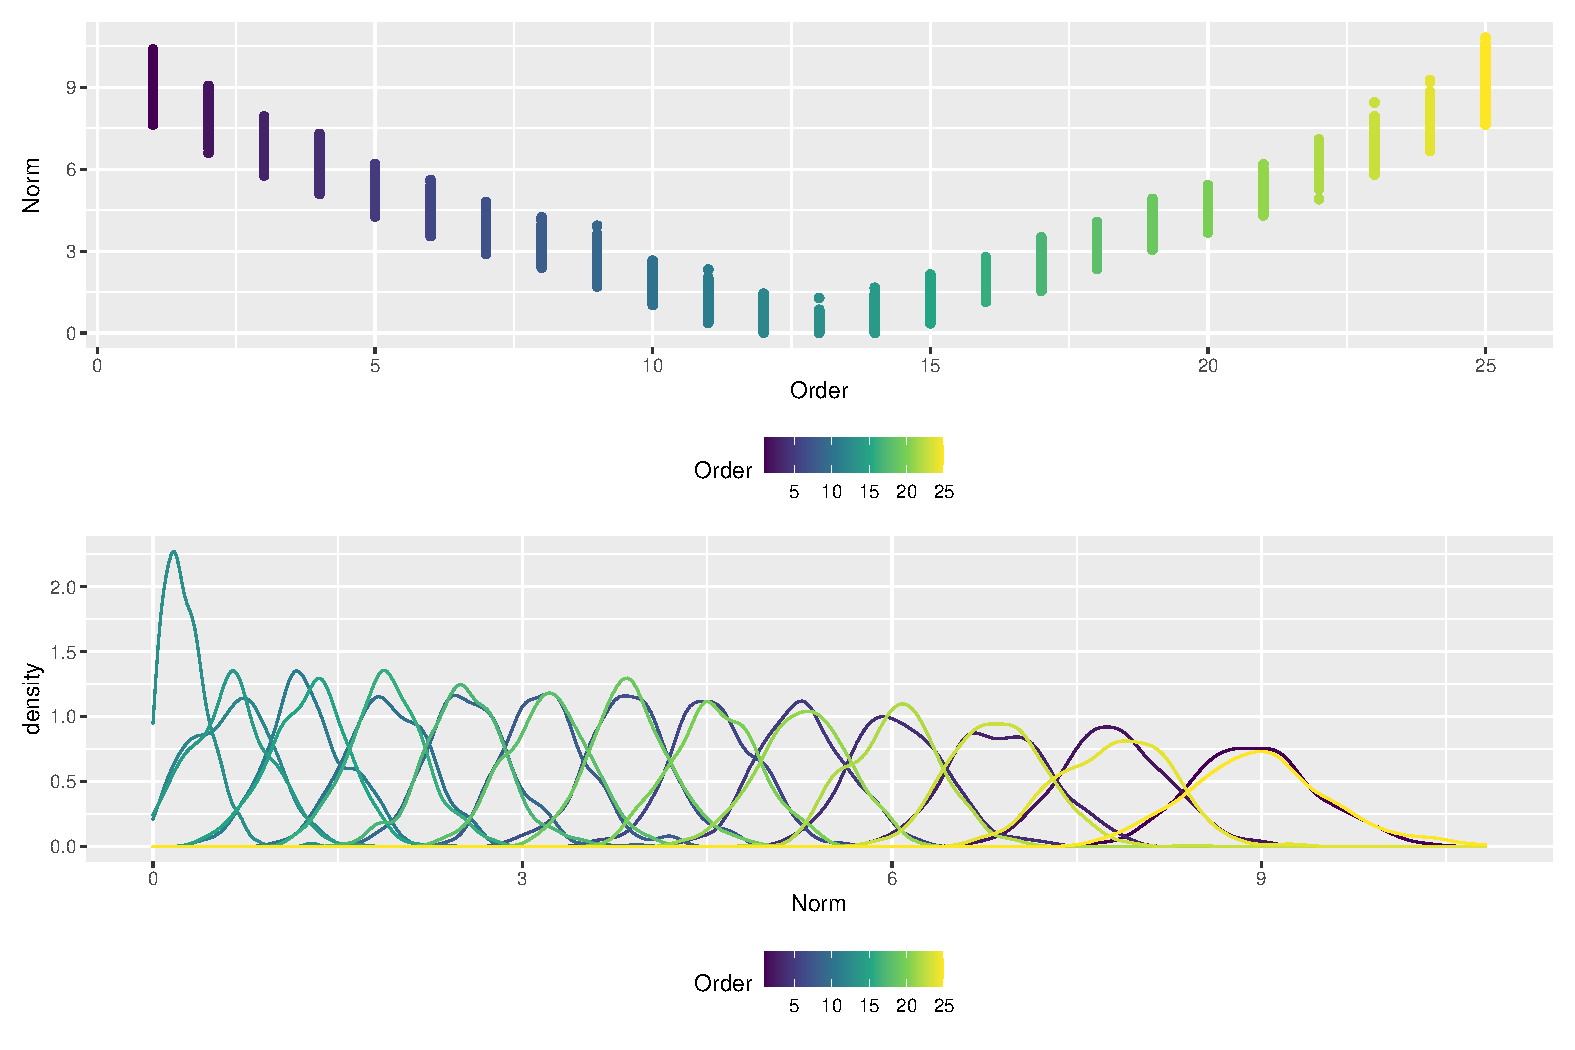
\includegraphics[scale = #2]{../graphics/chap4/4-2_Norm_spec}
    \caption{Wigner's Surmise for non-standard Beta Ensembles}
   \end{center}
   \label{beta_norm_spec}
  \end{figure}
}

\newcommand{\FIGUREbetaREsummary}[2]{
  \begin{figure}[#1]
   \begin{center}
    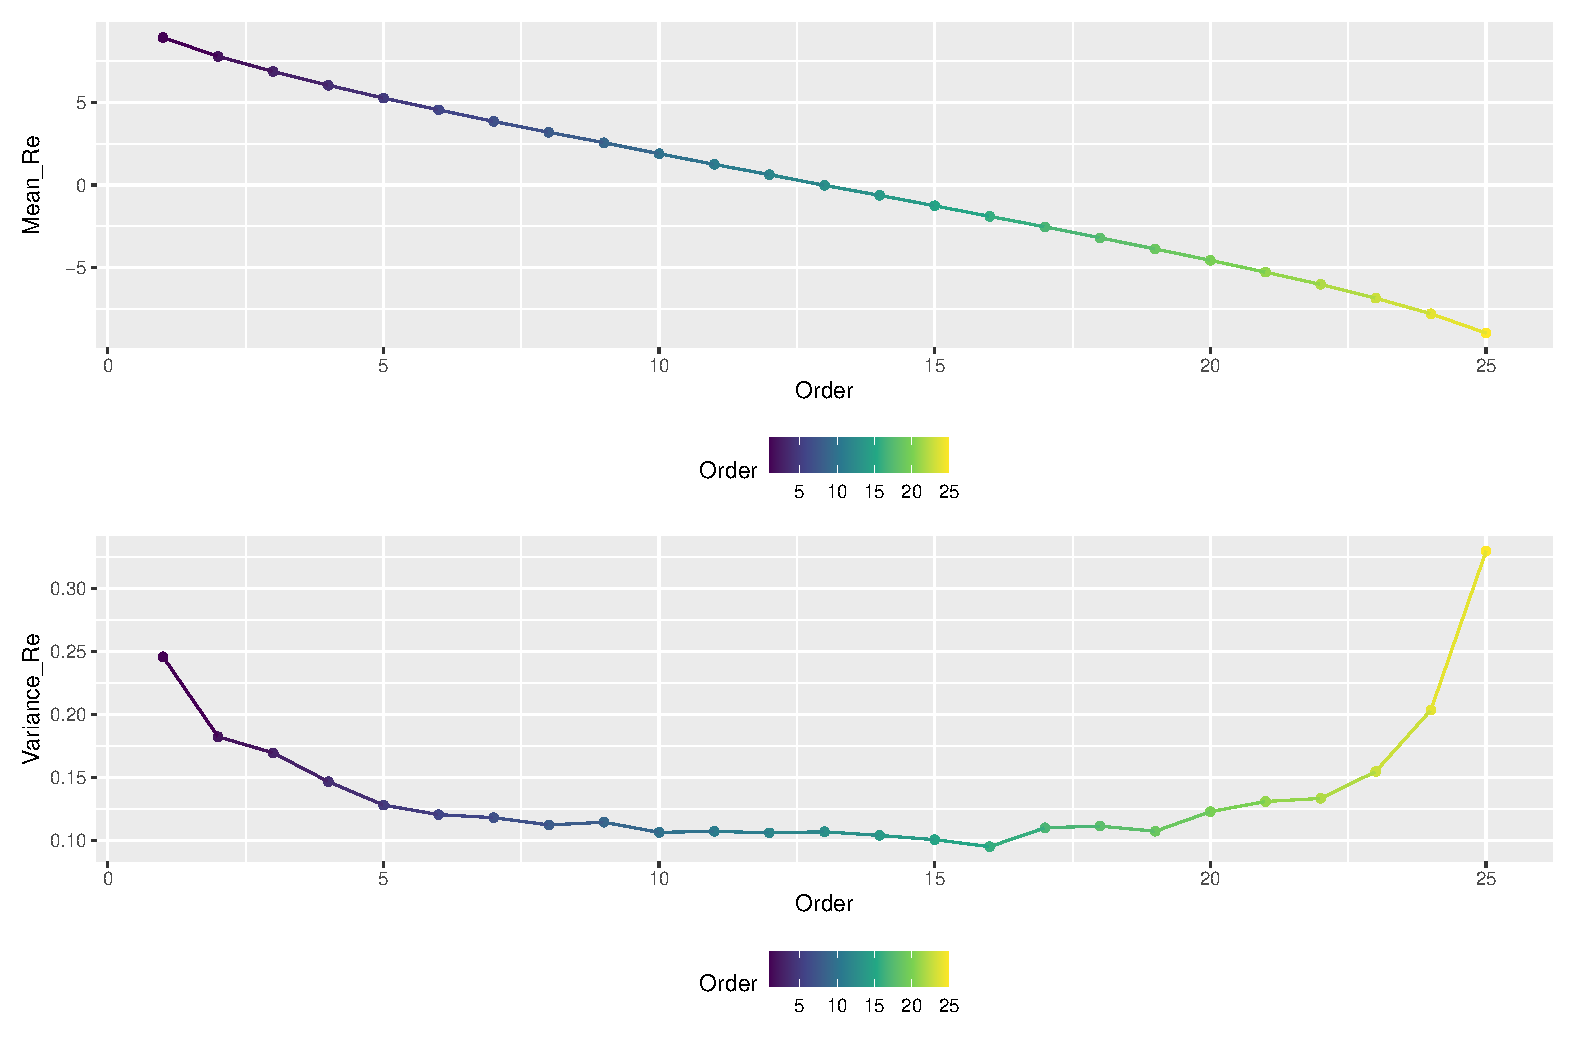
\includegraphics[scale = #2]{../graphics/chap4/4-2_Re_summary}
    \caption{Wigner's Surmise for non-standard Beta Ensembles}
   \end{center}
   \label{beta_re_summary}
  \end{figure}
}

\newcommand{\FIGUREbetaNORMsummary}[2]{
  \begin{figure}[#1]
   \begin{center}
    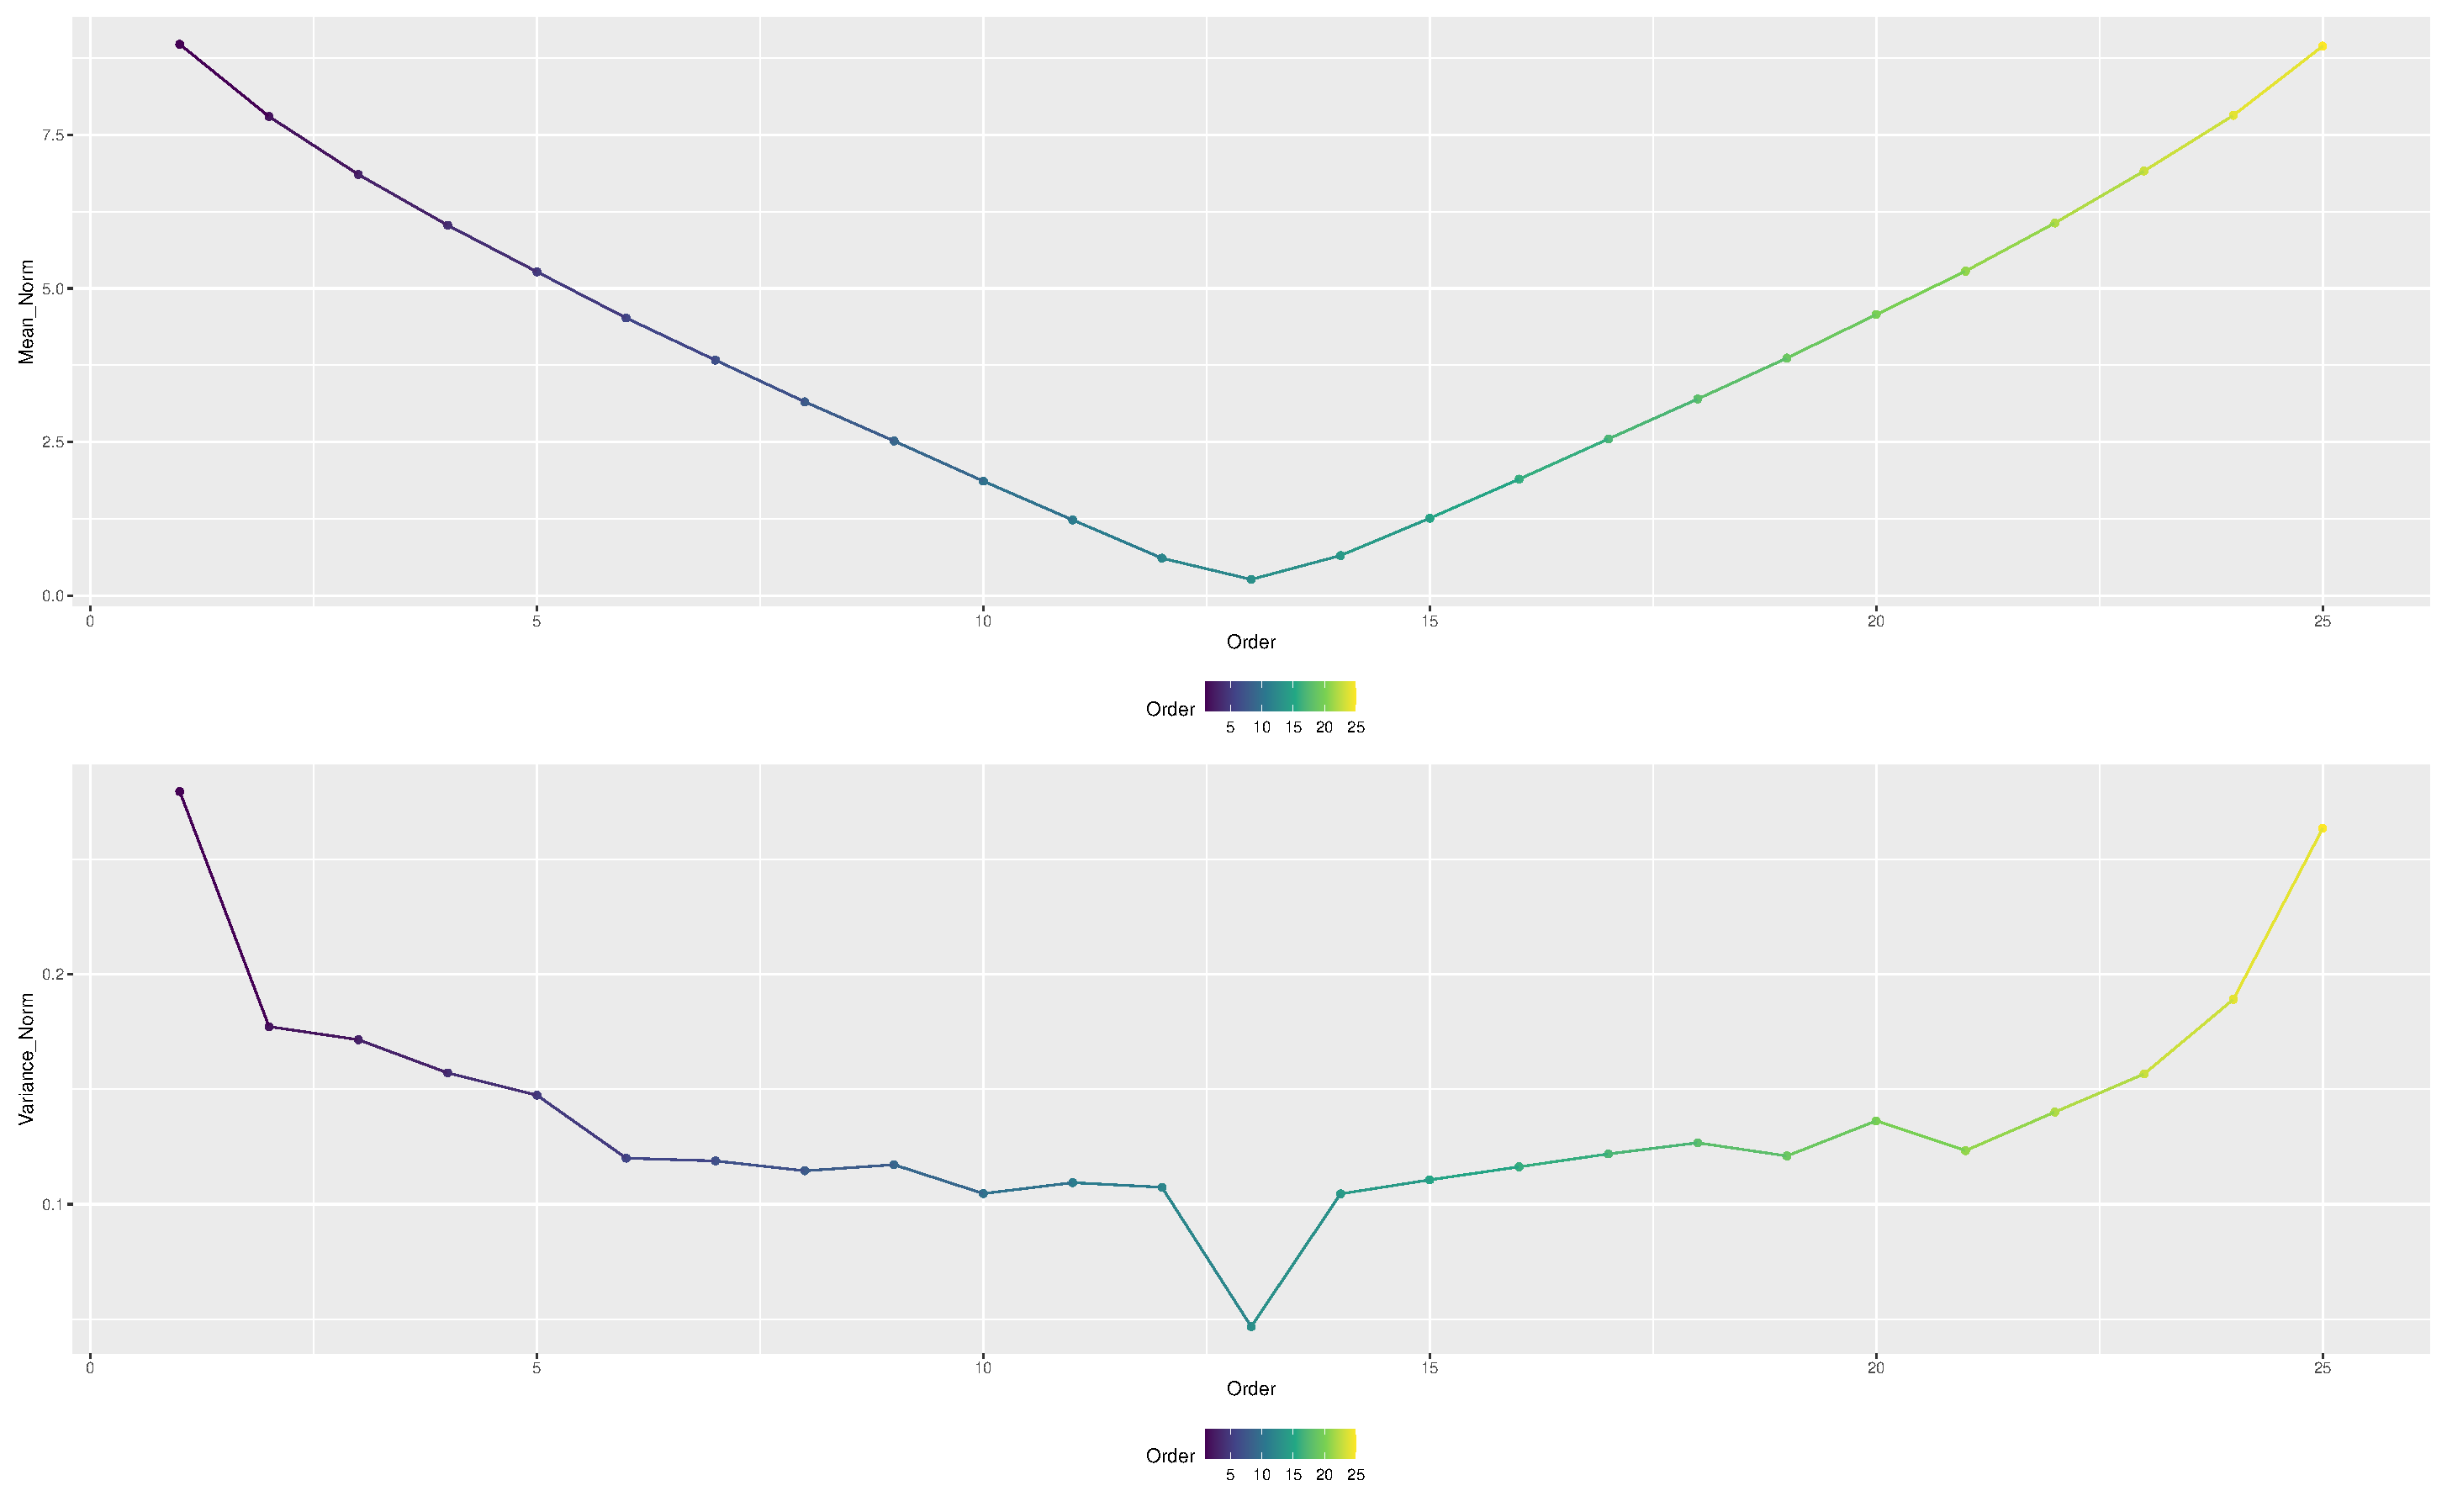
\includegraphics[scale = #2]{../graphics/chap4/4-2_Norm_summary}
    \caption{Wigner's Surmise for non-standard Beta Ensembles}
   \end{center}
   \label{beta_norm_summary}
  \end{figure}
}

\newcommand{\FIGUREsigbetaNORMspec}[2]{
  \begin{figure}[#1]
   \begin{center}
    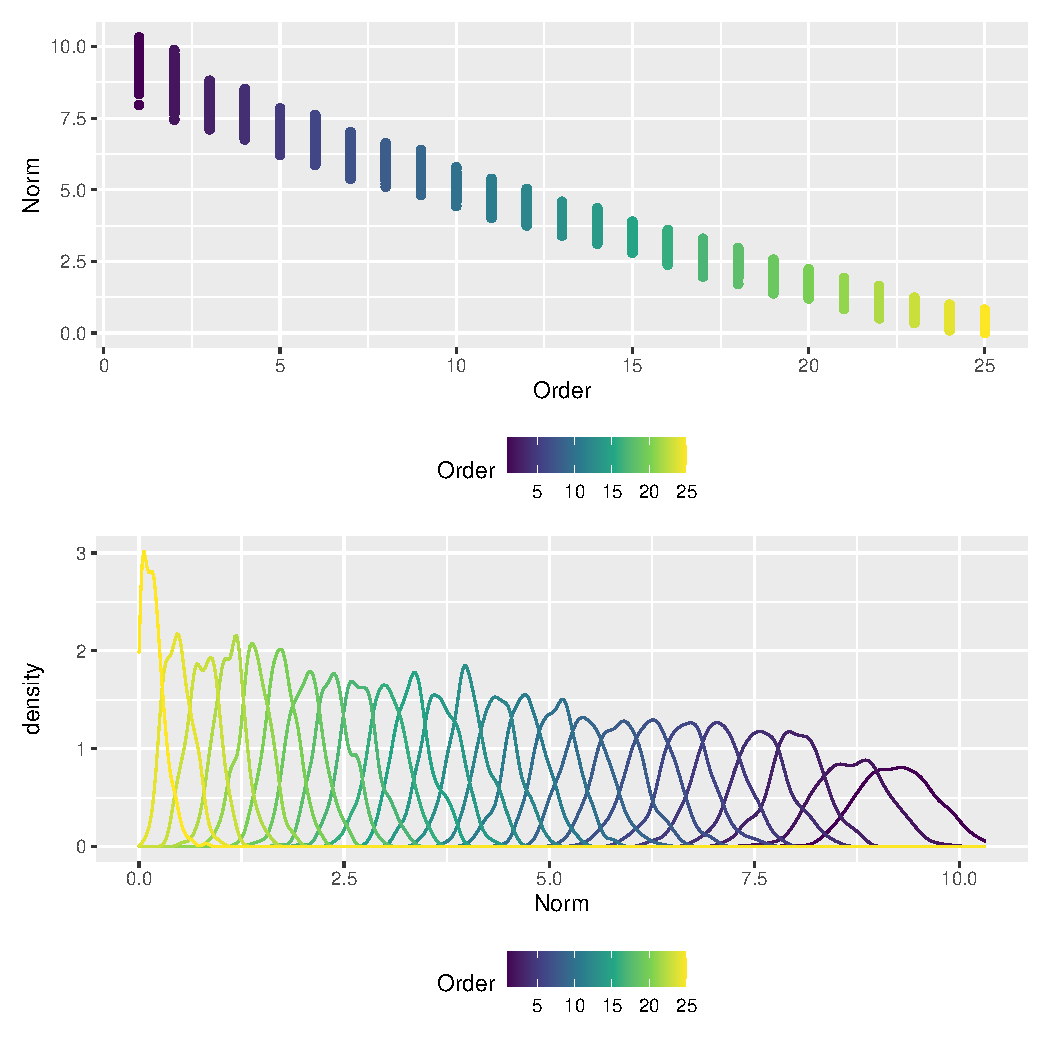
\includegraphics[scale = #2]{../graphics/chap4/4-2_SING_Norm_spec}
    \caption{Wigner's Surmise for non-standard Beta Ensembles}
   \end{center}
   \label{sig_beta_norm_spec}
  \end{figure}
}

\newcommand{\FIGUREsigbetaNORMsummary}[2]{
  \begin{figure}[#1]
   \begin{center}
    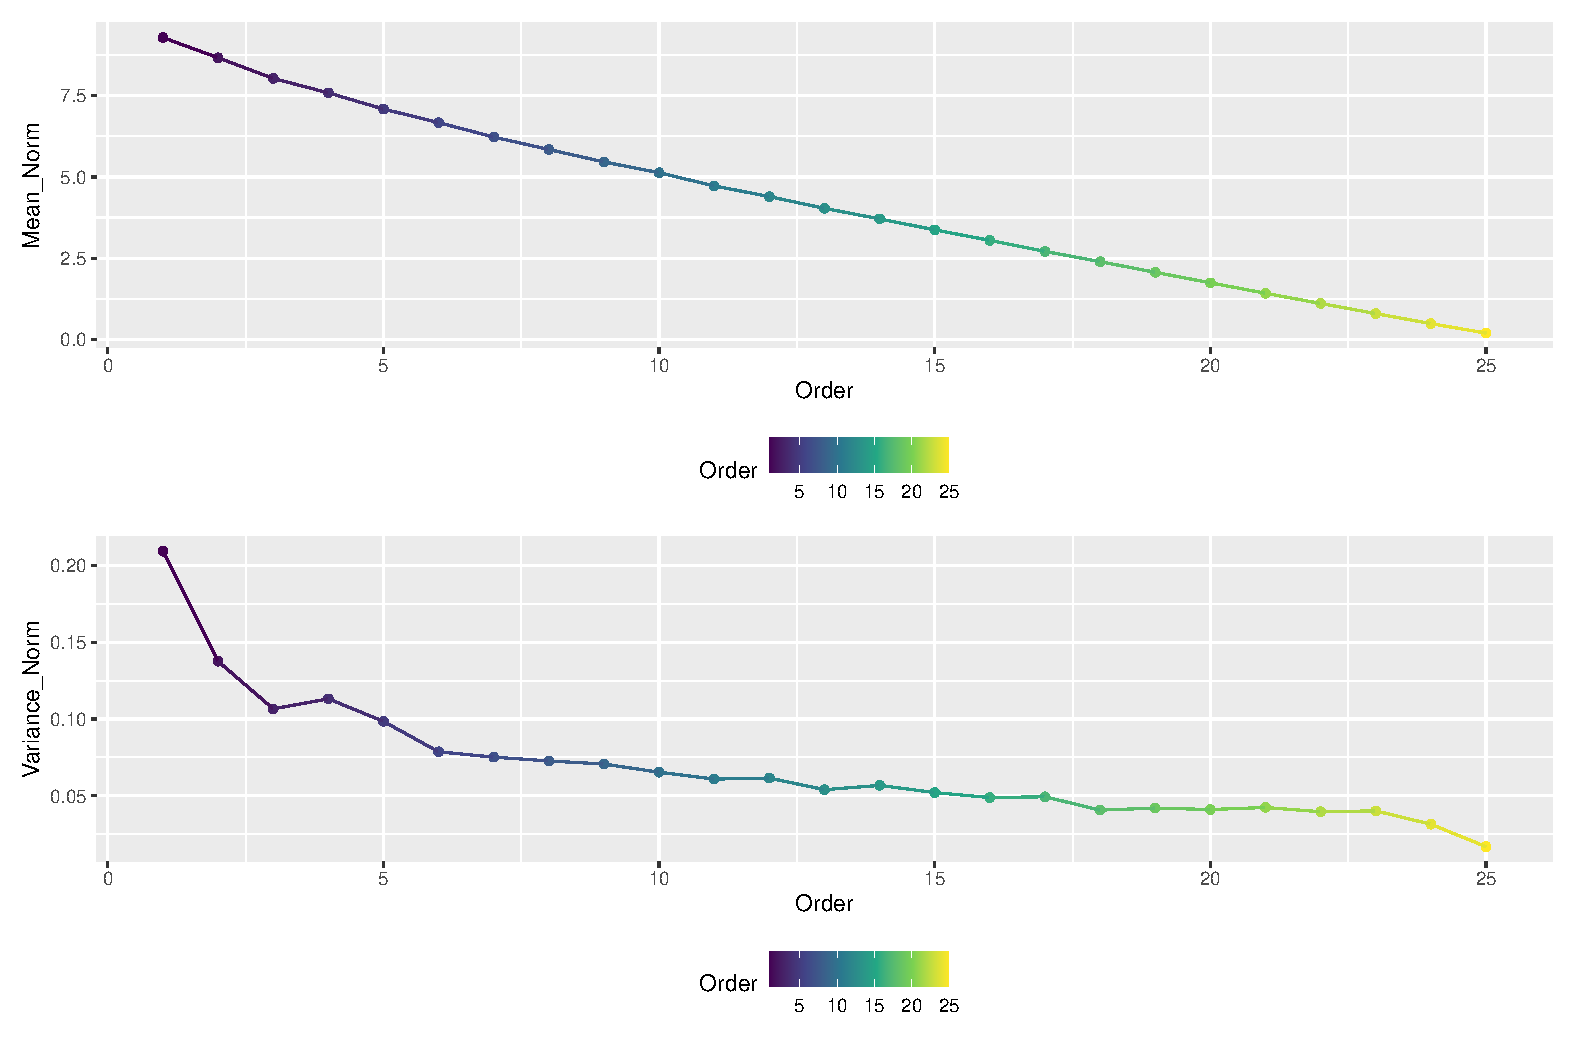
\includegraphics[scale = #2]{../graphics/chap4/4-2_SING_Norm_summary}
    \caption{Wigner's Surmise for non-standard Beta Ensembles}
   \end{center}
   \label{sig_beta_norm_summary}
  \end{figure}
}
